\documentclass[a4paper]{article}

\usepackage[english]{babel}
\usepackage[T1]{fontenc}
\usepackage{amsmath}
\usepackage{graphicx}
\usepackage[colorinlistoftodos]{todonotes}
\usepackage{makeidx}
\usepackage{fullpage,xspace,setspace,lscape}
\makeindex

\renewcommand{\thefigure}{S\arabic{figure}}


\title{\huge\bfseries \vspace{2cm} The \textit{E. coli} molecular phenotype under different growth conditions \\ \vspace{0.7cm}
	\Large\bfseries Supplementary materials \vspace{1.3cm}}


\author{
	\large\bfseries Mehmet U. Caglar*, John R. Houser, Craig S. Barnhart, \\
	\large\bfseries Daniel R. Boutz, Sean M. Carroll, Aurko Dasgupta, Walter F. Lenoir,\\ 
	\large\bfseries Bartram L. Smith, Viswanadham Sridhara, Dariya K. Sydykova, \\
	\large\bfseries Drew Vander Wood, Christopher J. Marx, \\
	\large\bfseries Edward M. Marcotte*, Jeffrey E. Barrick*, Claus O. Wilke*}


% allow floats to take up as much space as they want on a page
\renewcommand{\topfraction}{1.}	% max fraction of floats at top
\renewcommand{\bottomfraction}{1.}
\renewcommand{\textfraction}{0.}

\begin{document}
\maketitle
\newpage
	

\listoffigures


\newpage

\section*{Supplementary Figures}

\begin{figure}[!htb]
\centerline{	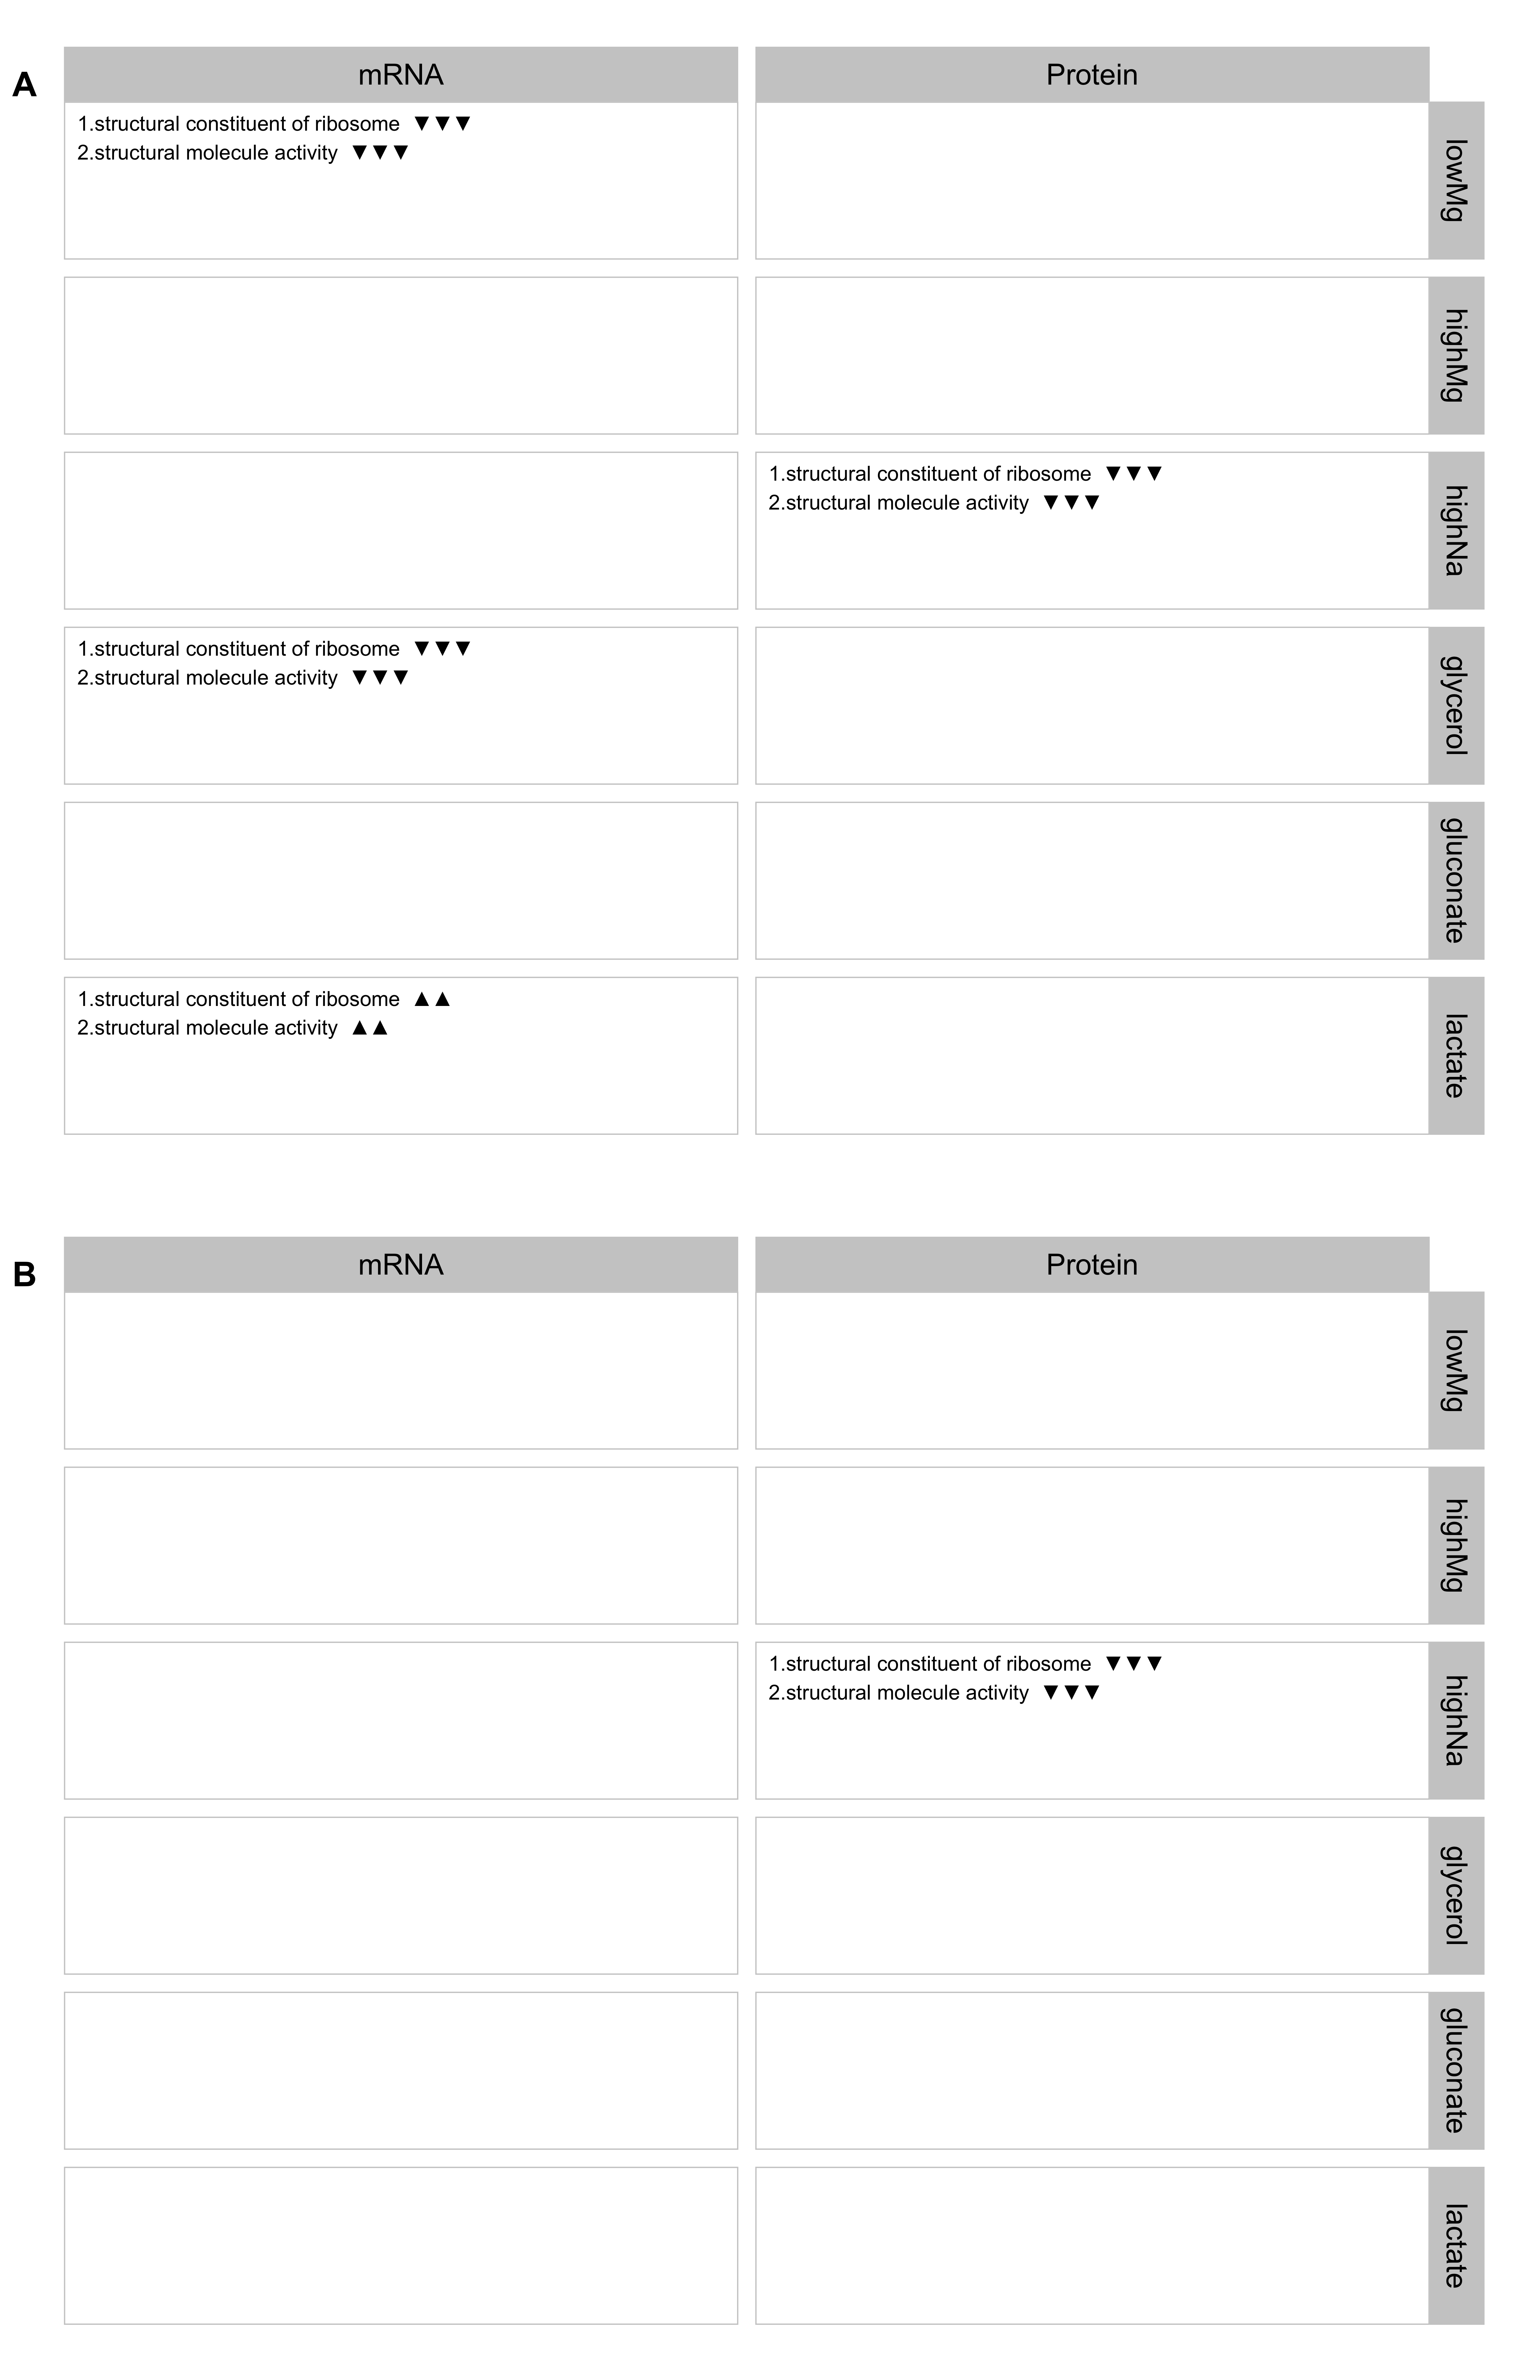
\includegraphics[width=0.7\textwidth]{../../d_figures/resultTable_mf.png}
}
	\caption[Significantly differentially expressed molecular functions]
	{\textbf{Significantly differentially expressed molecular functions, as determined by GO annotations.} For each condition, we show the top-5 differentially expressed molecular functions according to either mRNA or protein abundances.  Empty boxes indicate that no differentially expressed pathways were found. The arrows next to pathway names indicate the proportion of up- and down-regulated genes among the significantly differentially expressed genes in this pathway. One up arrow indicates that 60\% or more of the genes are up-regulated, two arrows correspond to 80\% or more genes, and three arrows correspond to 95\% or more genes being up-regulated. Similarly, down arrows indicate the proportion of down-regulated genes. (A) Exponential phase. (B) Stationary phase.}
\end{figure}

\clearpage

\begin{figure}[!htb]
	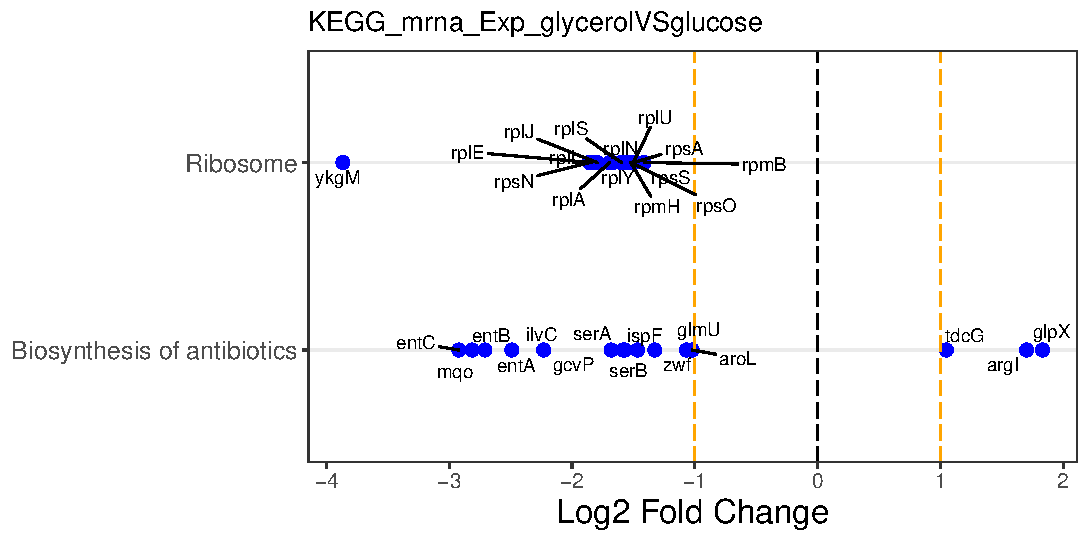
\includegraphics[width=1.0\textwidth]{../../d_figures/KEGG01_mrna_Exp_glycerolVSglucose_withTitle.pdf}
	\caption[Significantly differentially expressed KEGG pathways for mRNA samples in exponential phase tested for glycerol against glucose]
	{\textbf{Significantly differentially expressed KEGG pathways and associated genes with glycerol as carbon source, as determined by mRNA abundances in exponential phase.} The top 2 differentially expressed KEGG pathways are shown along the $y$ axis, and the relative fold change of the corresponding genes is shown along the $x$ axis. We show up to 10 of the most significantly changed pathways and for each pathway we show up to 15 of the most significantly changing genes.}
\end{figure}

\clearpage
\begin{figure}
	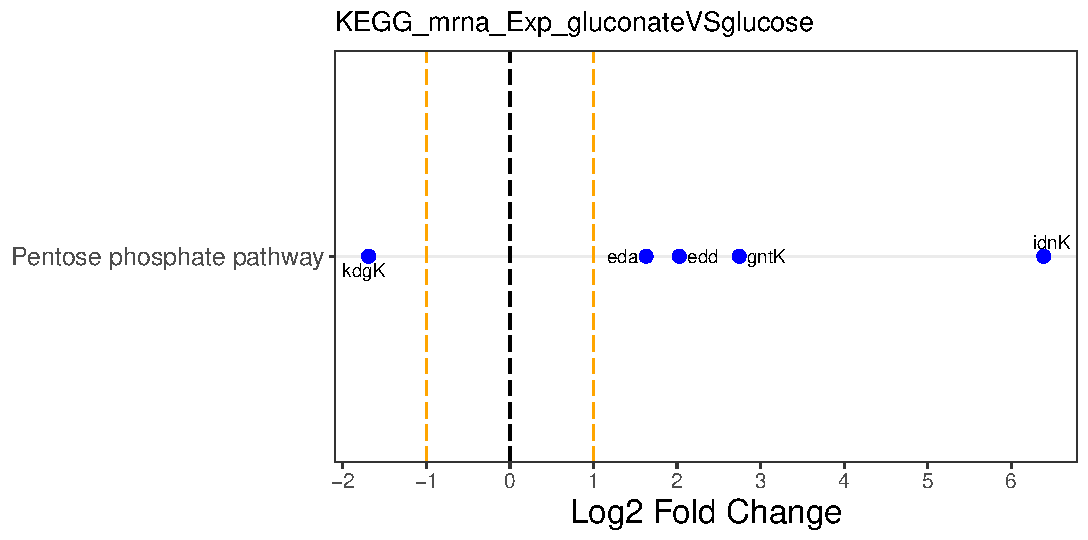
\includegraphics[width=1.0\textwidth]{../../d_figures/KEGG02_mrna_Exp_gluconateVSglucose_withTitle.pdf}
	\caption[Significantly differentially expressed KEGG pathways for mRNA samples in exponential phase tested for gluconate against glucose]
	{\textbf{Significantly differentially expressed KEGG pathway and associated genes with gluconate as carbon source, as determined by mRNA abundances in exponential phase.} The top differentially expressed KEGG pathway is shown along the $y$ axis, and the relative fold change of the corresponding genes is shown along the $x$ axis. We show up to 10 of the most significantly changed pathways and for each pathway we show up to 15 of the most significantly changing genes.}
\end{figure}

\clearpage
\begin{figure}
	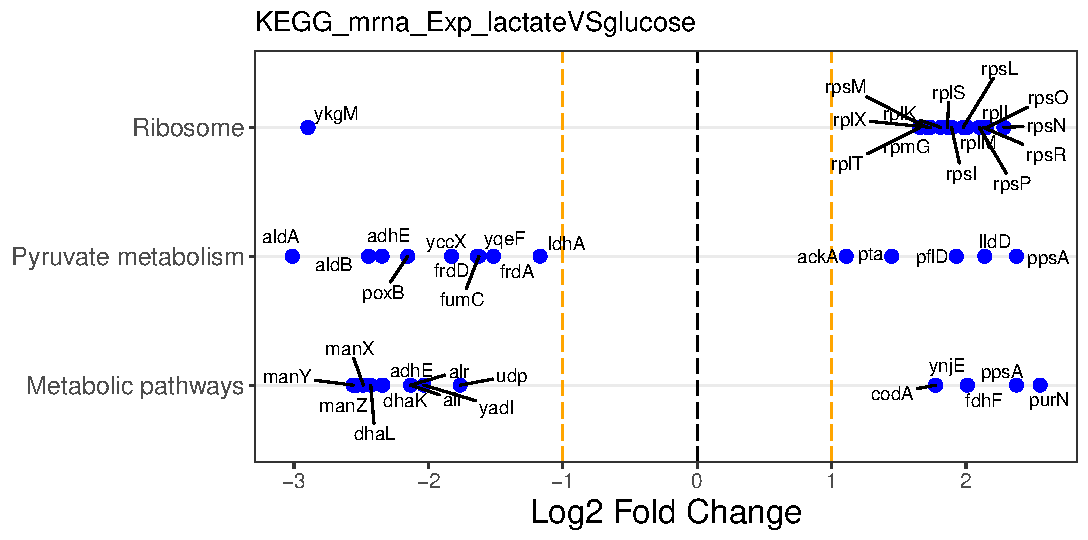
\includegraphics[width=1.0\textwidth]{../../d_figures/KEGG03_mrna_Exp_lactateVSglucose_withTitle.pdf}
	\caption[Significantly differentially expressed KEGG pathways for mRNA samples in exponential phase tested for lactate against glucose]
	{\textbf{Significantly differentially expressed KEGG pathways and associated genes with lactate as carbon source, as determined by mRNA abundances in exponential phase.} The top 3 differentially expressed KEGG pathways are shown along the $y$ axis, and the relative fold change of the corresponding genes is shown along the $x$ axis. We show up to 10 of the most significantly changed pathways and for each pathway we show up to 15 of the most significantly changing genes.}
\end{figure}

\clearpage
\begin{figure}
	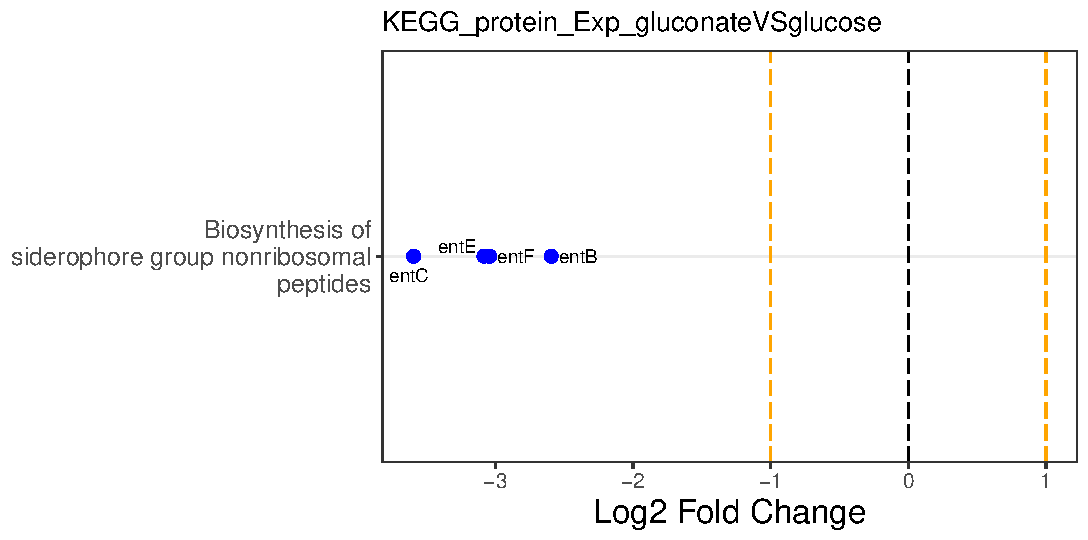
\includegraphics[width=1.0\textwidth]{../../d_figures/KEGG04_protein_Exp_gluconateVSglucose_withTitle.pdf}
	\caption[Significantly differentially expressed KEGG pathway for protein samples in exponential phase tested for gluconate against glucose]
	{\textbf{Significantly differentially expressed KEGG pathway and associated genes with gluconate as carbon source, as determined by protein abundances in exponential phase.} The top differentially expressed KEGG pathway is shown along the $y$ axis, and the relative fold change of the corresponding genes is shown along the $x$ axis. We show up to 10 of the most significantly changed pathways and for each pathway we show up to 15 of the most significantly changing genes.}
\end{figure}

\clearpage
\begin{figure}
	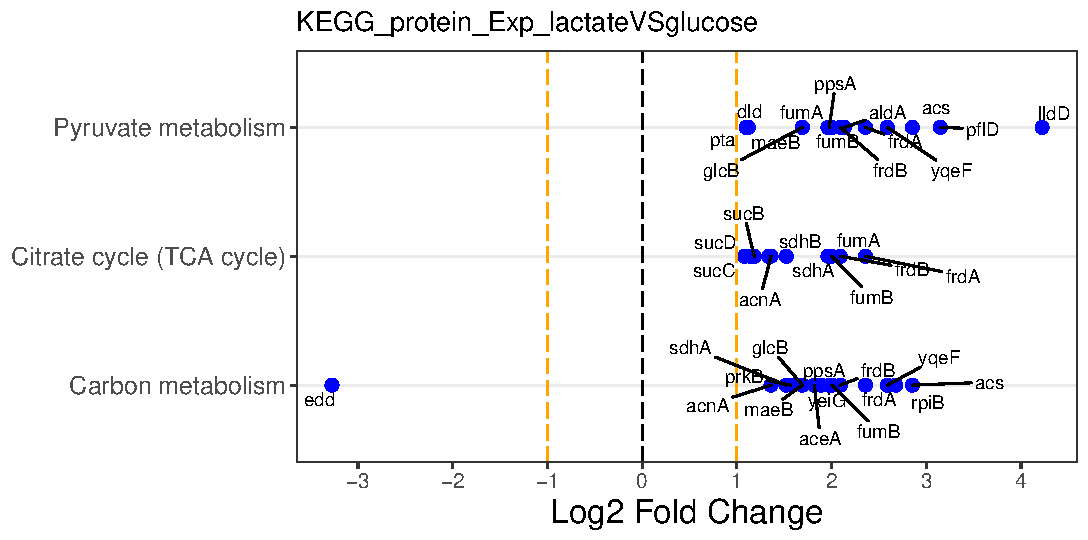
\includegraphics[width=1.0\textwidth]{../../d_figures/KEGG05_protein_Exp_lactateVSglucose_withTitle.pdf}
	\caption[Significantly differentially expressed KEGG pathways for protein samples in exponential phase tested for lactate against glucose]
	{\textbf{Significantly differentially expressed KEGG pathways and associated genes with lactate as carbon source, as determined by protein abundances in exponential phase.} The top 3 differentially expressed KEGG pathways are shown along the $y$ axis, and the relative fold change of the corresponding genes is shown along the $x$ axis. We show up to 10 of the most significantly changed pathways and for each pathway we show up to 15 of the most significantly changing genes.}
\end{figure}

\clearpage
\begin{figure}
	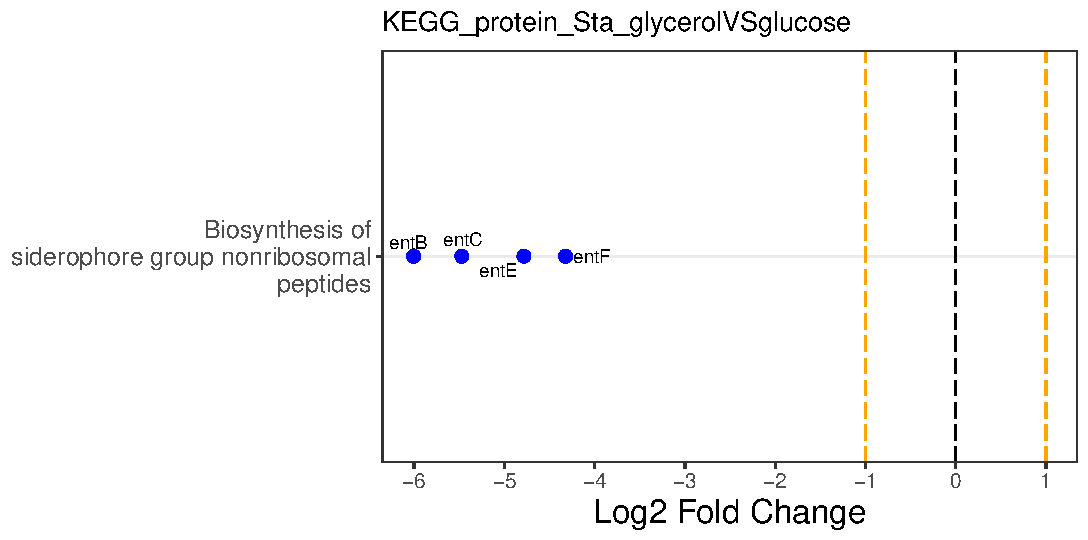
\includegraphics[width=1.0\textwidth]{../../d_figures/KEGG06_protein_Sta_glycerolVSglucose_withTitle.pdf}
	\caption[Significantly differentially expressed KEGG pathway for protein samples in stationary phase tested for glycerol against glucose]
	{\textbf{Significantly differentially expressed KEGG pathway and associated genes with glycerol as carbon source, as determined by protein abundances in stationary phase.} The top differentially expressed KEGG pathway is shown along the $y$ axis, and the relative fold change of the corresponding genes is shown along the $x$ axis. We show up to 10 of the most significantly changed pathways and for each pathway, we show up to 15 of the most significantly changing genes.}
\end{figure}

\clearpage
\begin{figure}
	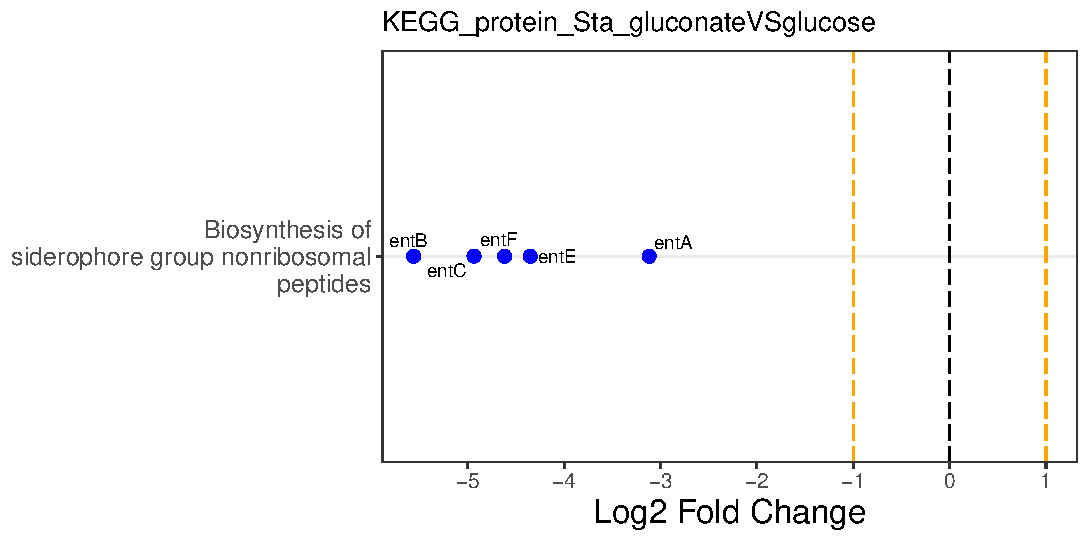
\includegraphics[width=1.0\textwidth]{../../d_figures/KEGG07_protein_Sta_gluconateVSglucose_withTitle.pdf}
	\caption[Significantly differentially expressed KEGG pathway for protein samples in stationary phase tested for gluconate against glucose]
	{\textbf{Significantly differentially expressed KEGG pathway and associated genes with gluconate as carbon source, as determined by protein abundances in stationary phase.} The top differentially expressed KEGG pathway is shown along the $y$ axis, and the relative fold change of the corresponding genes is shown along the $x$ axis. We show up to 10 of the most significantly changed pathways and for each pathway, we show up to 15 of the most significantly changing genes.}
\end{figure}

\clearpage
\begin{figure}
	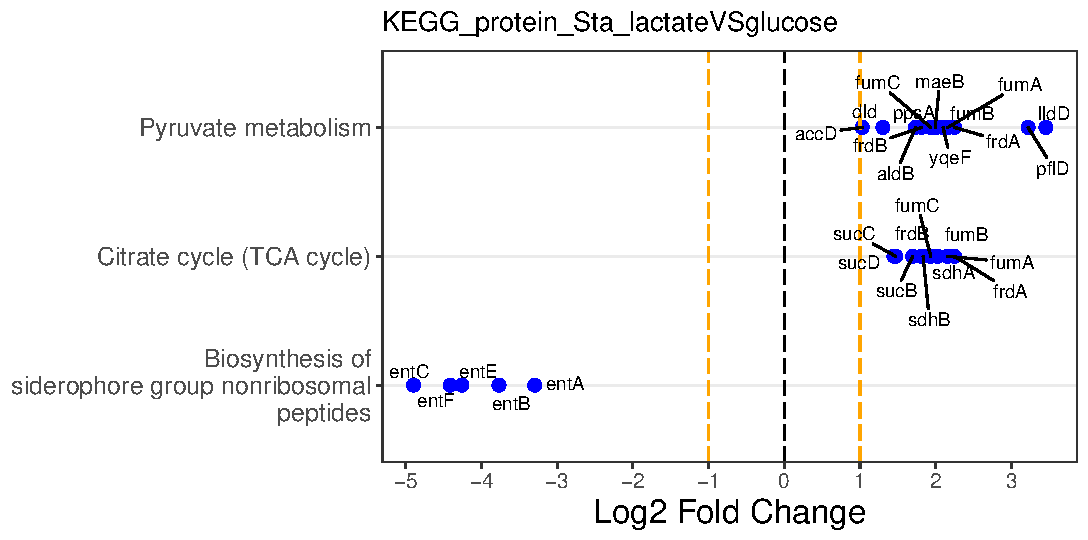
\includegraphics[width=1.0\textwidth]{../../d_figures/KEGG08_protein_Sta_lactateVSglucose_withTitle.pdf}
	\caption[Significantly differentially expressed KEGG pathways for protein samples in stationary phase tested for lactate against glucose]
	{\textbf{Significantly differentially expressed KEGG pathways and associated genes with lactate as carbon source, as determined by protein abundances in stationary phase.} The top 3 differentially expressed KEGG pathways are shown along the $y$ axis, and the relative fold change of the corresponding genes is shown along the $x$ axis. We show up to 10 of the most significantly changed pathways and for each pathway, we show up to 15 of the most significantly changing genes.}
\end{figure}

\clearpage
\begin{figure}
	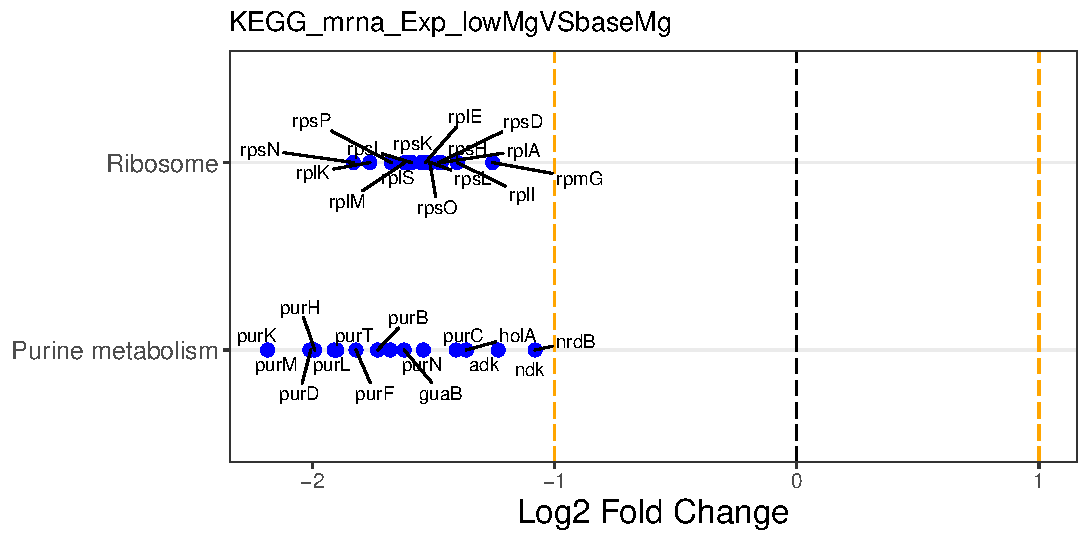
\includegraphics[width=1.0\textwidth]{../../d_figures/KEGG09_mrna_Exp_lowMgVSbaseMg_withTitle.pdf}
	\caption[Significantly differentially expressed KEGG pathways for mRNA samples in exponential phase tested for low Mg\textsuperscript{2+} levels against base Mg\textsuperscript{2+}]
	{\textbf{Significantly differentially expressed KEGG pathways and associated genes with low Mg\textsuperscript{2+} levels, as determined by mRNA abundances in exponential phase.} The top 2 differentially expressed KEGG pathways are shown along the $y$ axis, and the relative fold change of the corresponding genes is shown along the $x$ axis. We show up to 10 of the most significantly changed pathways and for each pathway, we show up to 15 of the most significantly changing genes.}
\end{figure}

\clearpage
\begin{figure}
	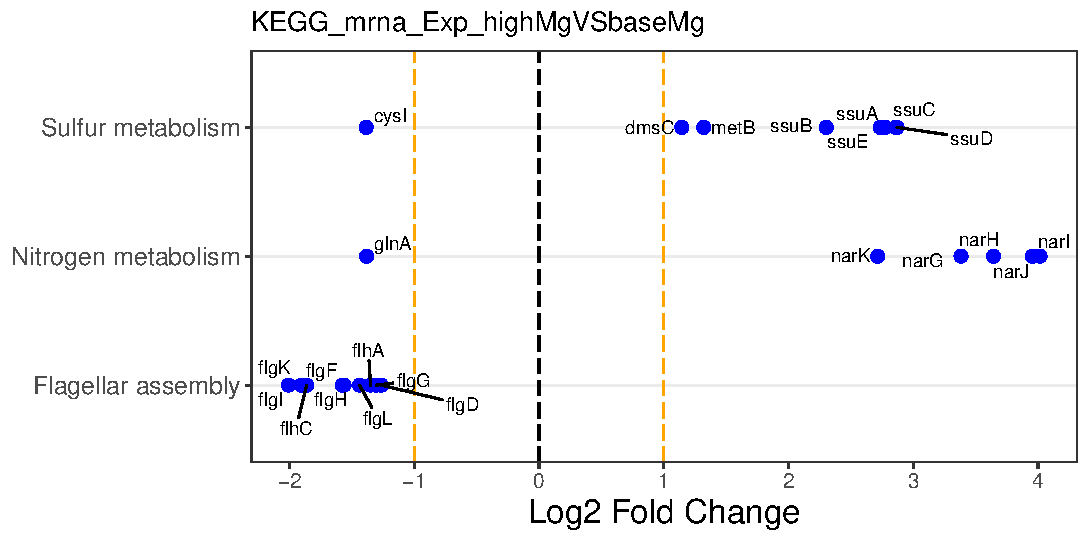
\includegraphics[width=1.0\textwidth]{../../d_figures/KEGG10_mrna_Exp_highMgVSbaseMg_withTitle.pdf}
	\caption[Significantly differentially expressed KEGG pathways for mRNA samples in exponential phase tested for high Mg\textsuperscript{2+} against base Mg\textsuperscript{2+}]
	{\textbf{Significantly differentially expressed KEGG pathways and associated genes with high Mg\textsuperscript{2+} levels, as determined by mRNA abundances in exponential phase.} The top 3 differentially expressed KEGG pathways are shown along the $y$ axis, and the relative fold change of the corresponding genes is shown along the $x$ axis. We show up to 10 of the most significantly changed pathways and for each pathway, we show up to 15 of the most significantly changing genes.}
\end{figure}

\clearpage
\begin{figure}
	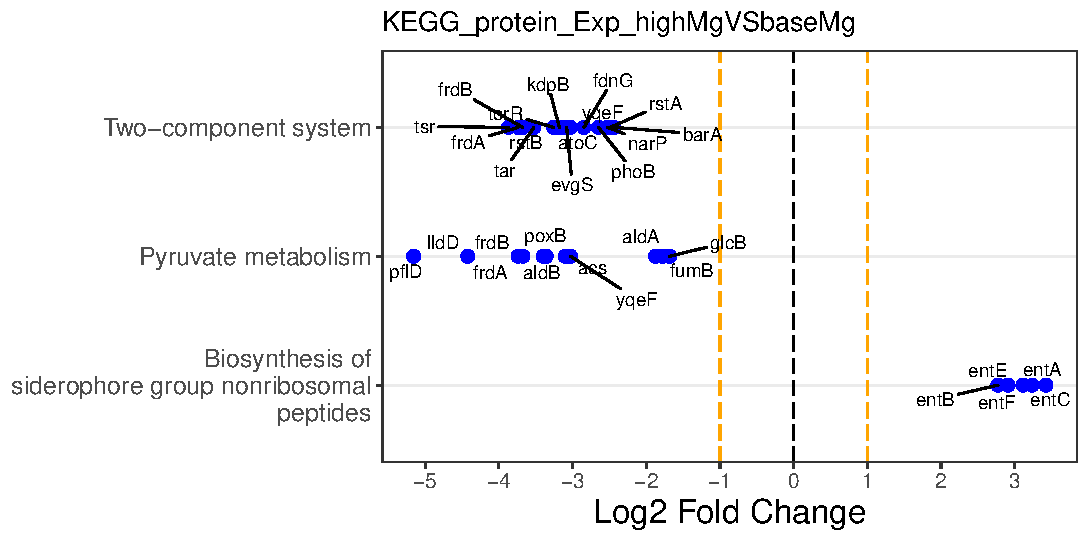
\includegraphics[width=1.0\textwidth]{../../d_figures/KEGG11_protein_Exp_highMgVSbaseMg_withTitle.pdf}
	\caption[Significantly differentially expressed KEGG pathways for protein samples in exponential phase tested for high Mg\textsuperscript{2+} against base Mg\textsuperscript{2+}]
	{\textbf{Significantly differentially expressed KEGG pathways and associated genes with high Mg\textsuperscript{2+} levels, as determined by protein abundances in exponential phase.} The top 3 differentially expressed KEGG pathways are shown along the $y$ axis, and the relative fold change of the corresponding genes is shown along the $x$ axis. We show up to 10 of the most significantly changed pathways and for each pathway, we show up to 15 of the most significantly changing genes.}
\end{figure}

\clearpage
\begin{figure}
	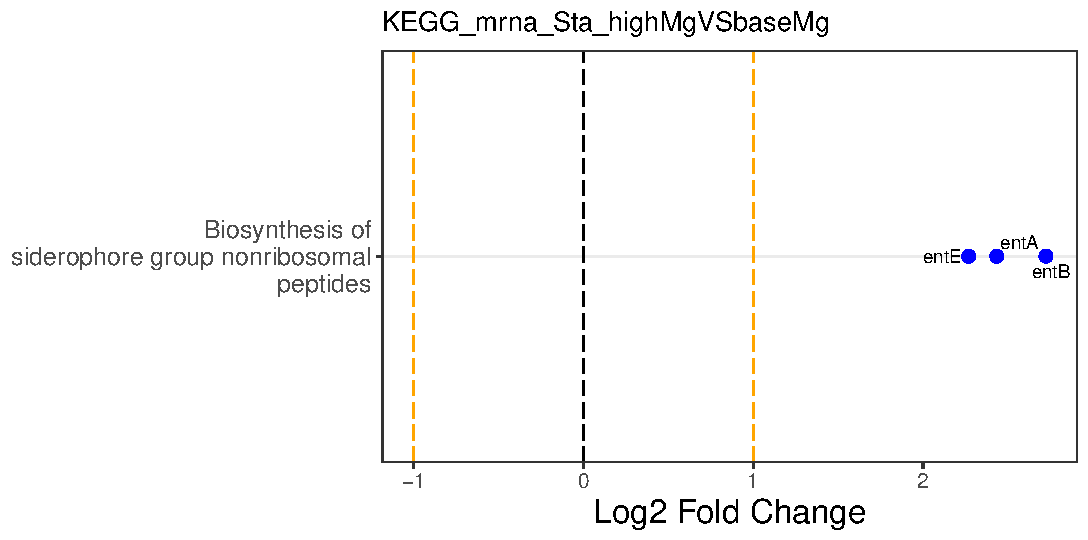
\includegraphics[width=1.0\textwidth]{../../d_figures/KEGG12_mrna_Sta_highMgVSbaseMg_withTitle.pdf}
	\caption[Significantly differentially expressed KEGG pathway for mRNA samples in stationary phase tested for high Mg\textsuperscript{2+} against base Mg\textsuperscript{2+}]
	{\textbf{Significantly differentially expressed KEGG pathway and associated genes with high Mg\textsuperscript{2+} levels, as determined by mRNA abundances in stationary phase.} The top differentially expressed KEGG pathway is shown along the $y$ axis, and the relative fold change of the corresponding genes is shown along the $x$ axis. We show up to 10 of the most significantly changed pathways and for each pathway, we show up to 15 of the most significantly changing genes.}
\end{figure}

\clearpage
\begin{figure}
	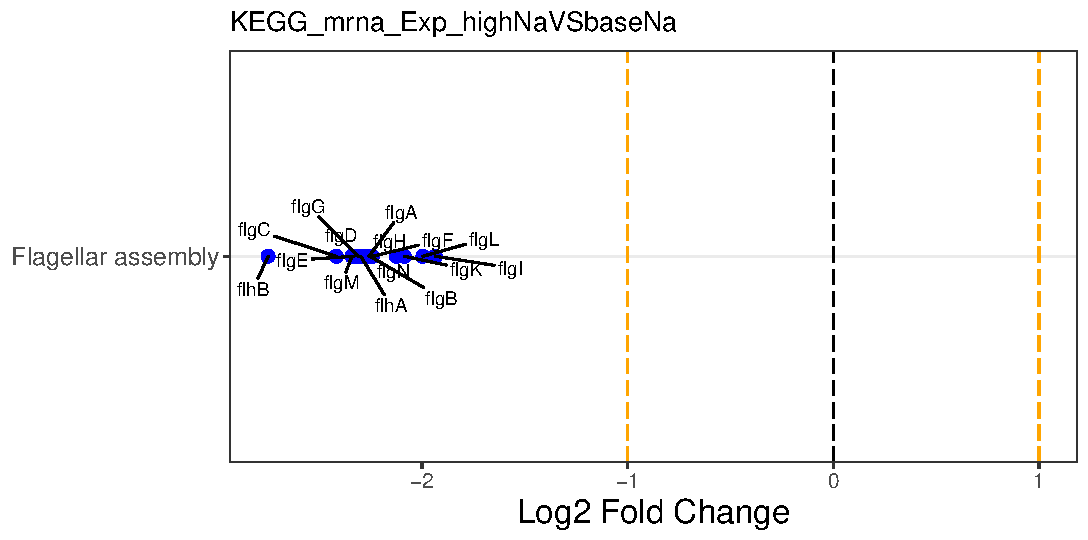
\includegraphics[width=1.0\textwidth]{../../d_figures/KEGG13_mrna_Exp_highNaVSbaseNa_withTitle.pdf}
	\caption[Significantly differentially expressed KEGG pathway for mRNA samples in exponential phase tested for high Na\textsuperscript{+} against base Na\textsuperscript{+}]
	{\textbf{Significantly differentially expressed KEGG pathway and associated genes with high Na\textsuperscript{+} levels, as determined by mRNA abundances in exponential phase.} The top differentially expressed KEGG pathway is shown along the $y$ axis, and the relative fold change of the corresponding genes is shown along the $x$ axis. We show up to 10 of the most significantly changed pathways and for each pathway, we show up to 15 of the most significantly changing genes.}
\end{figure}

\clearpage
\begin{figure}
	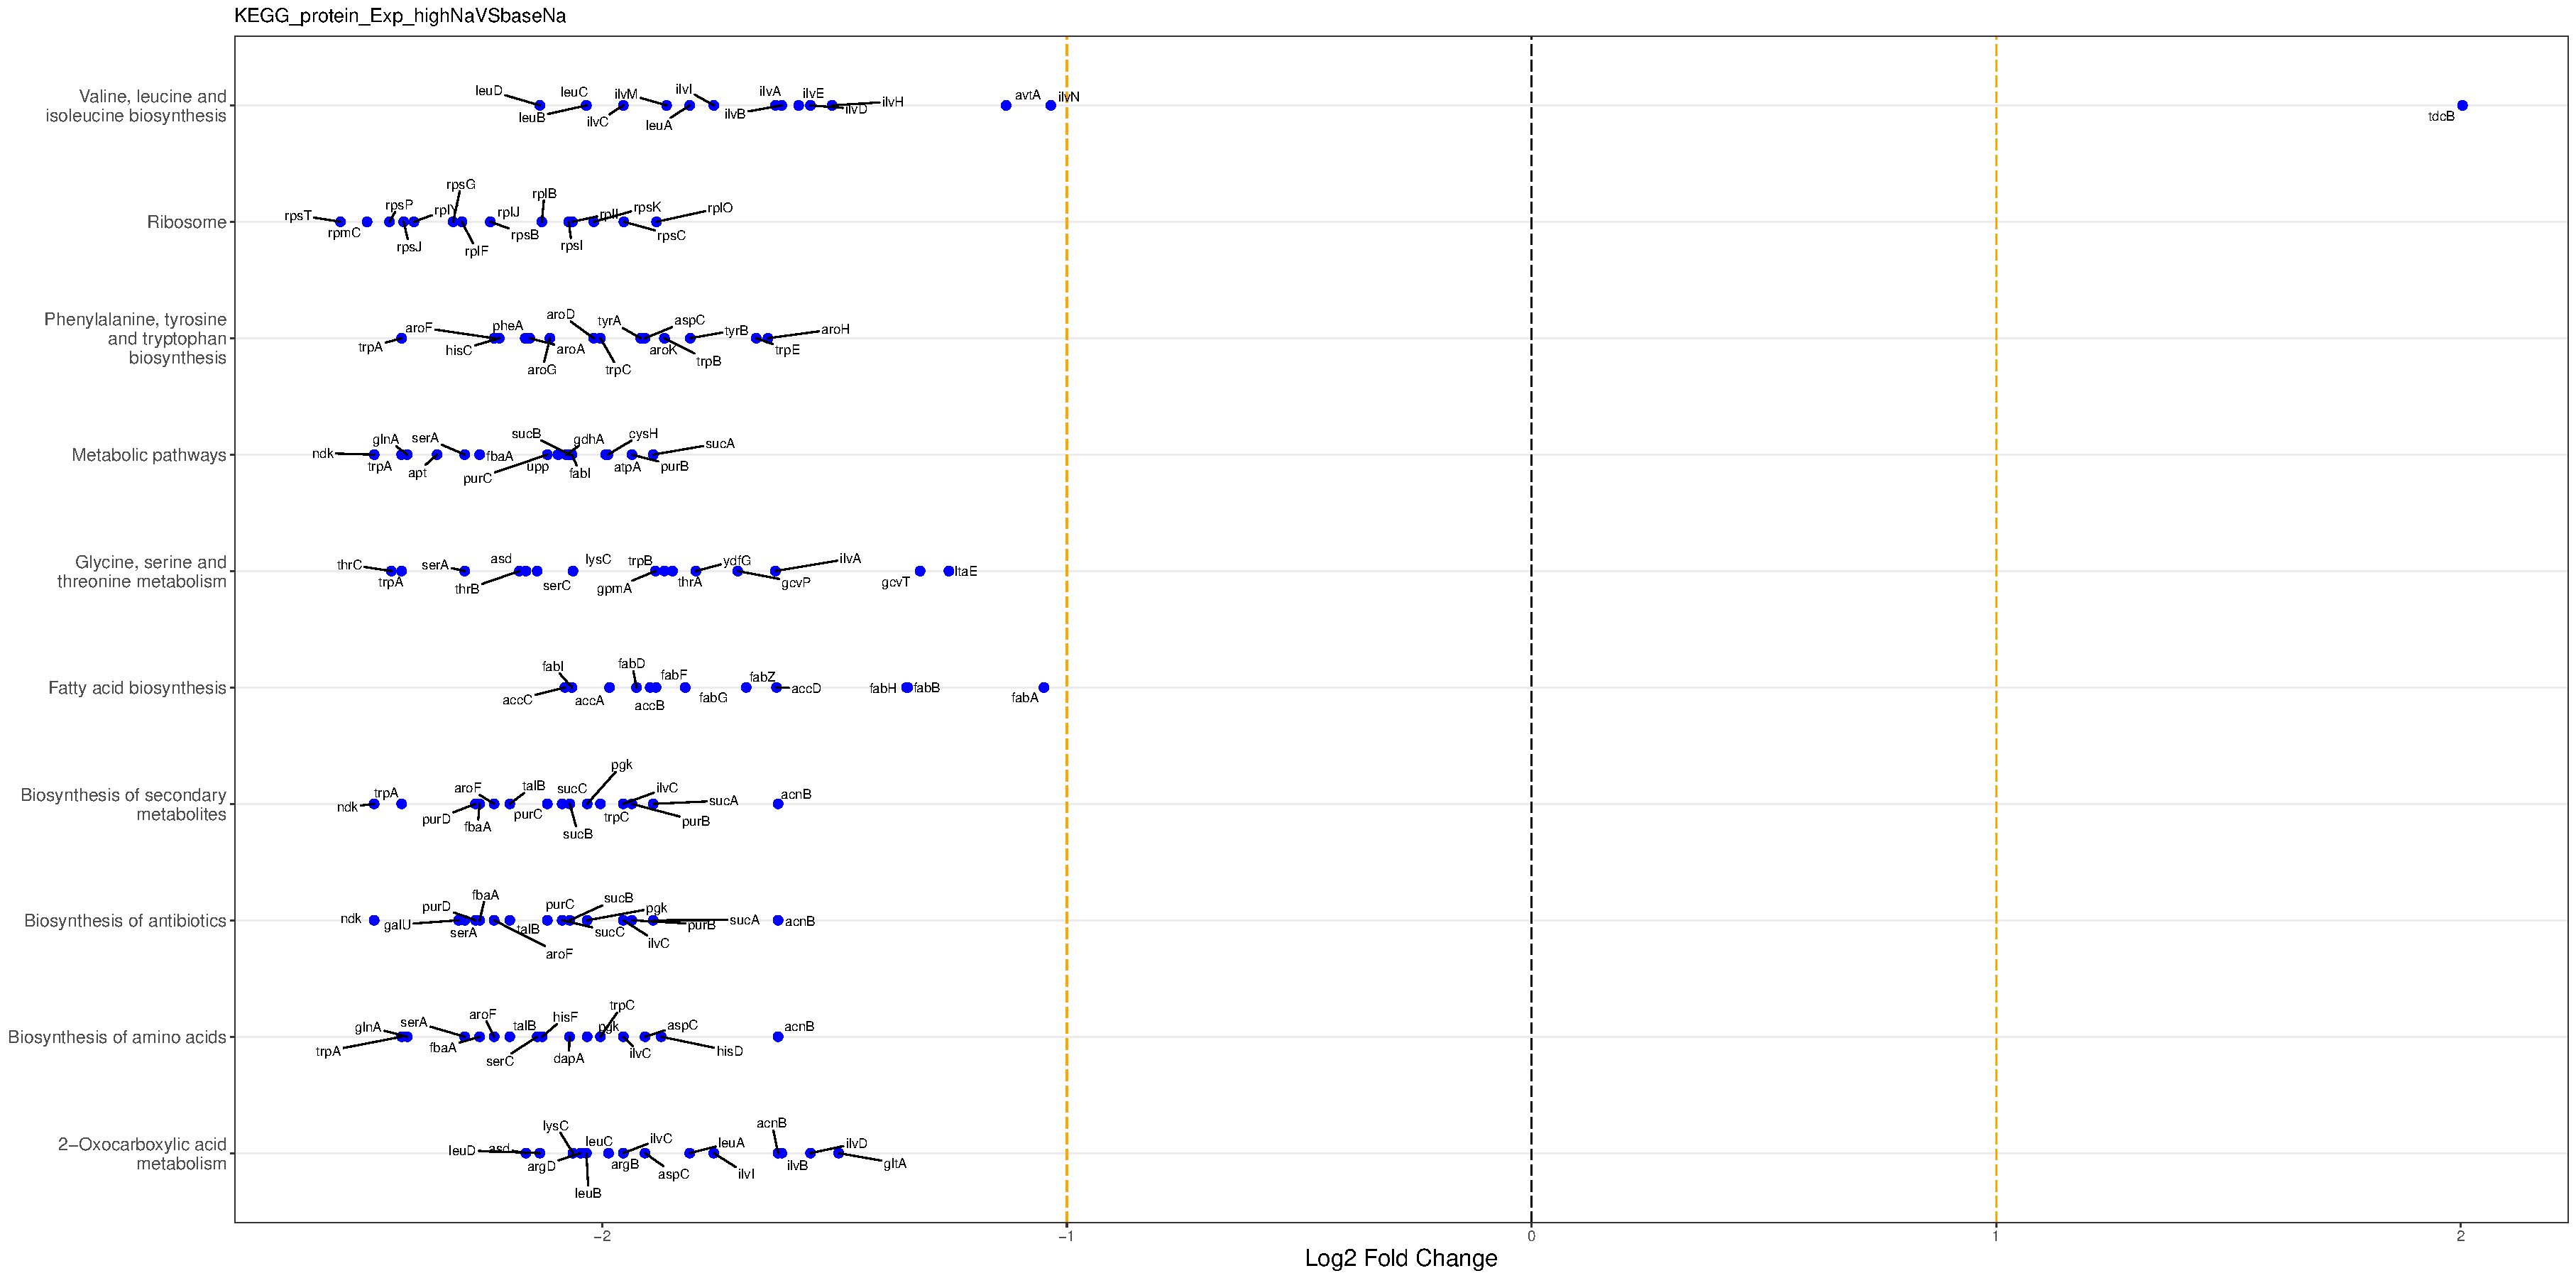
\includegraphics[width=1.0\textwidth]{../../d_figures/KEGG14_protein_Exp_highNaVSbaseNa_withTitle.pdf}
	\caption[Significantly differentially expressed KEGG pathways for protein samples in exponential phase tested for high Na\textsuperscript{+} against base Na\textsuperscript{+}]
	{\textbf{Significantly differentially expressed KEGG pathways and associated genes with high Na\textsuperscript{+} levels, as determined by protein abundances in exponential phase.} The top 10 differentially expressed KEGG pathways are shown along the $y$ axis, and the relative fold change of the corresponding genes is shown along the $x$ axis. We show up to 10 of the most significantly changed pathways and for each pathway, we show up to 15 of the most significantly changing genes.}
\end{figure}

\clearpage
\begin{figure}
	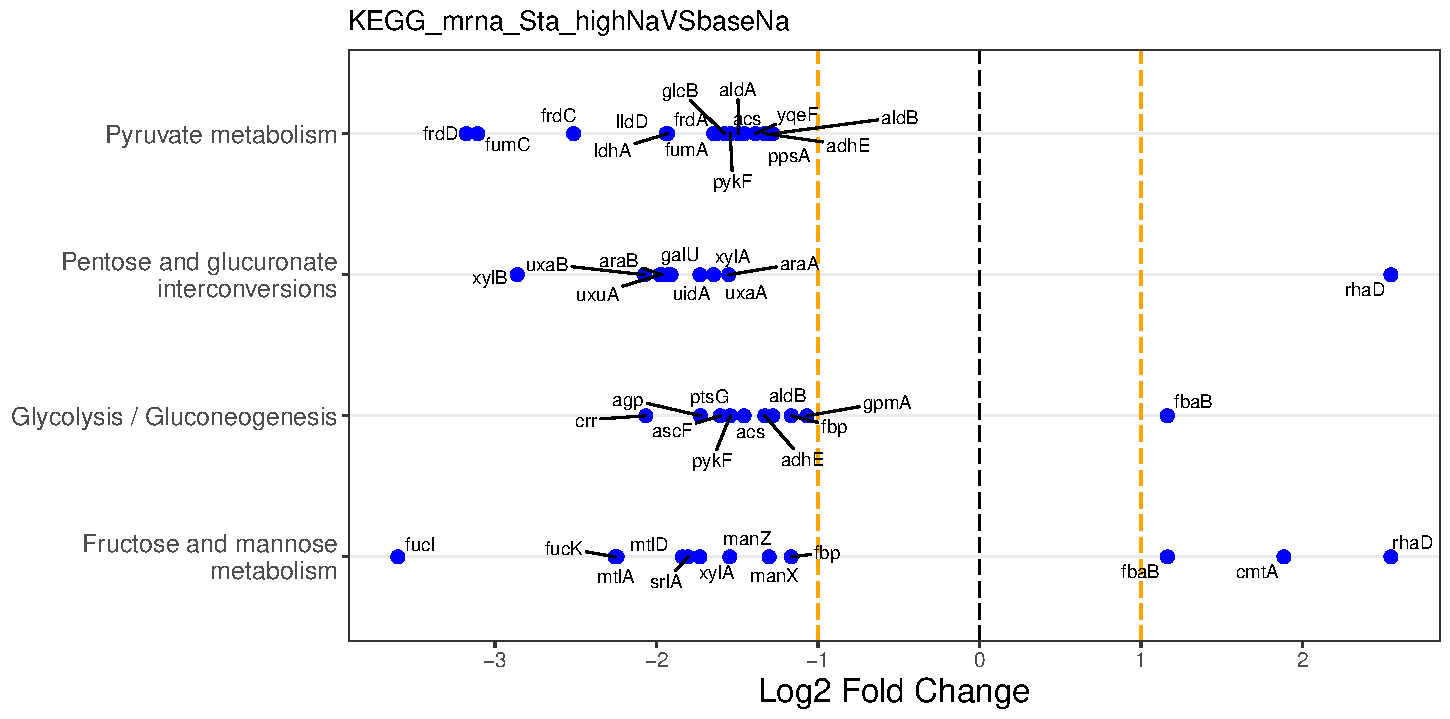
\includegraphics[width=1.0\textwidth]{../../d_figures/KEGG15_mrna_Sta_highNaVSbaseNa_withTitle.pdf}
	\caption[Significantly differentially expressed KEGG pathways for mRNA samples in stationary phase tested for high Na\textsuperscript{+} against base Na\textsuperscript{+}]
	{\textbf{Significantly differentially expressed KEGG pathways and associated genes with high Na\textsuperscript{+} levels, as determined by mRNA abundances in stationary phase.} The top 4 differentially expressed KEGG pathways are shown along the $y$ axis, and the relative fold change of the corresponding genes is shown along the $x$ axis. We show up to 10 of the most significantly changed pathways and for each pathway, we show up to 15 of the most significantly changing genes.}
\end{figure}

\clearpage
\begin{figure}
	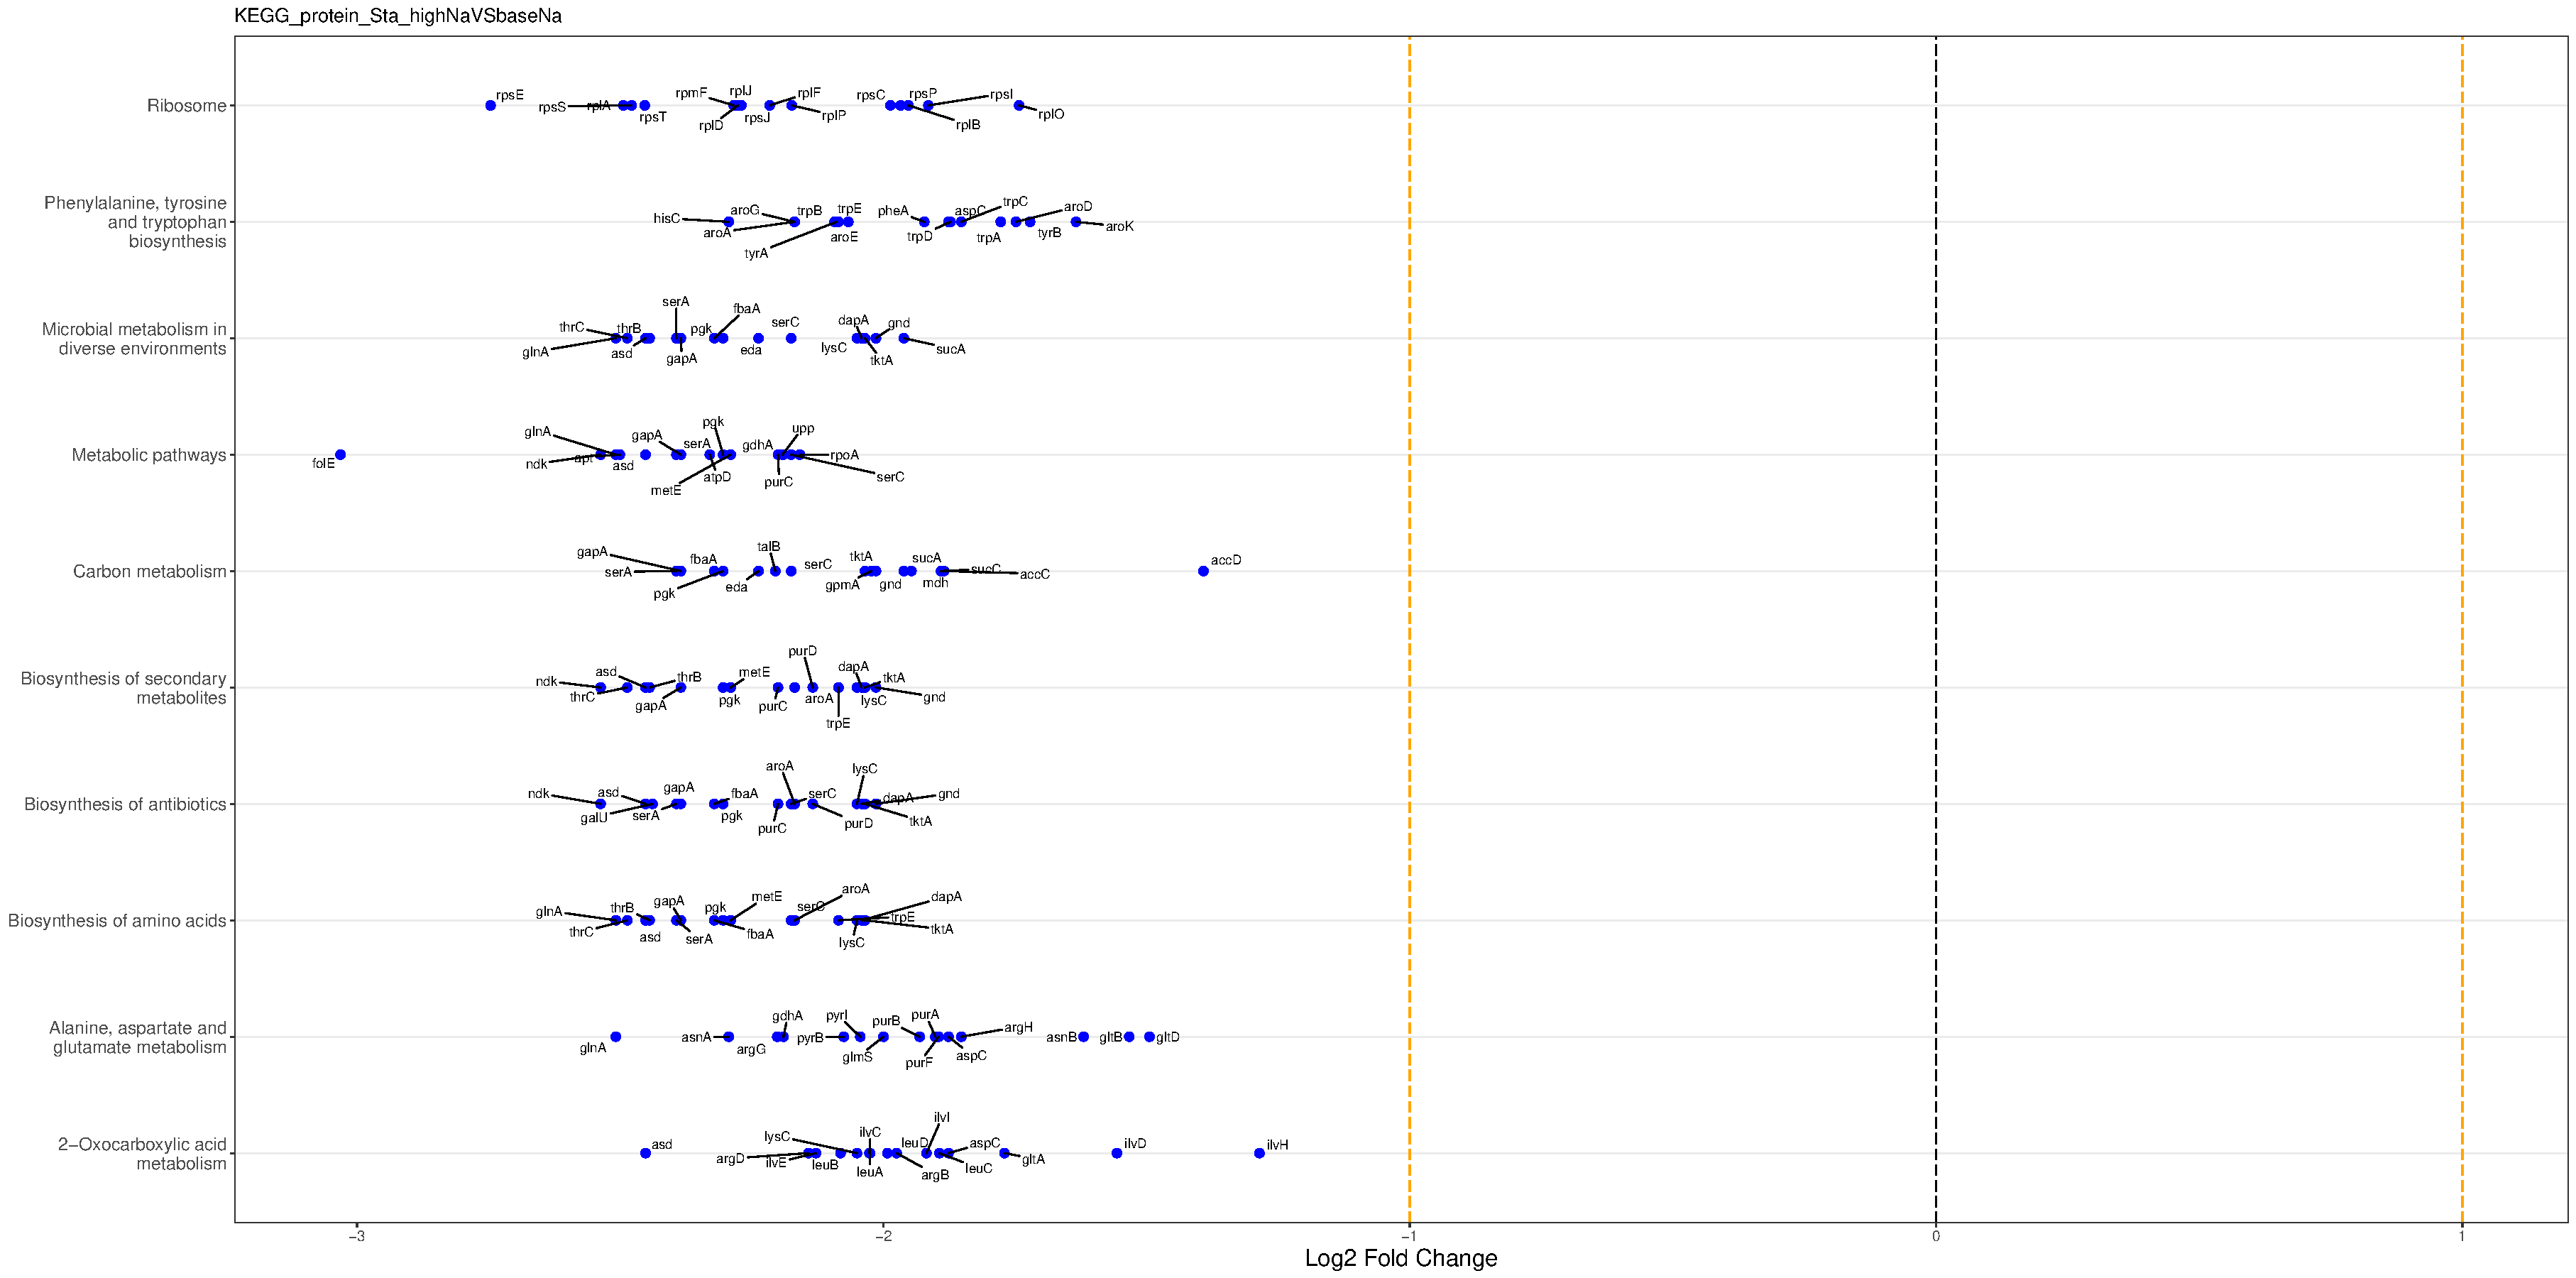
\includegraphics[width=1.0\textwidth]{../../d_figures/KEGG16_protein_Sta_highNaVSbaseNa_withTitle}
	\caption[Significantly differentially expressed KEGG pathways for protein samples in stationary phase tested for high Na\textsuperscript{+} against base Na\textsuperscript{+}]
	{\textbf{Significantly differentially expressed KEGG pathways and associated genes with high Na\textsuperscript{+} levels, as determined by protein abundances in stationary phase.} The top 10 differentially expressed KEGG pathways are shown along the $y$ axis, and the relative fold change of the corresponding genes is shown along the $x$ axis. We show up to 10 of the most significantly changed pathways and for each pathway, we show up to 15 of the most significantly changing genes.}
\end{figure}
\clearpage


\begin{figure}[!htb]
	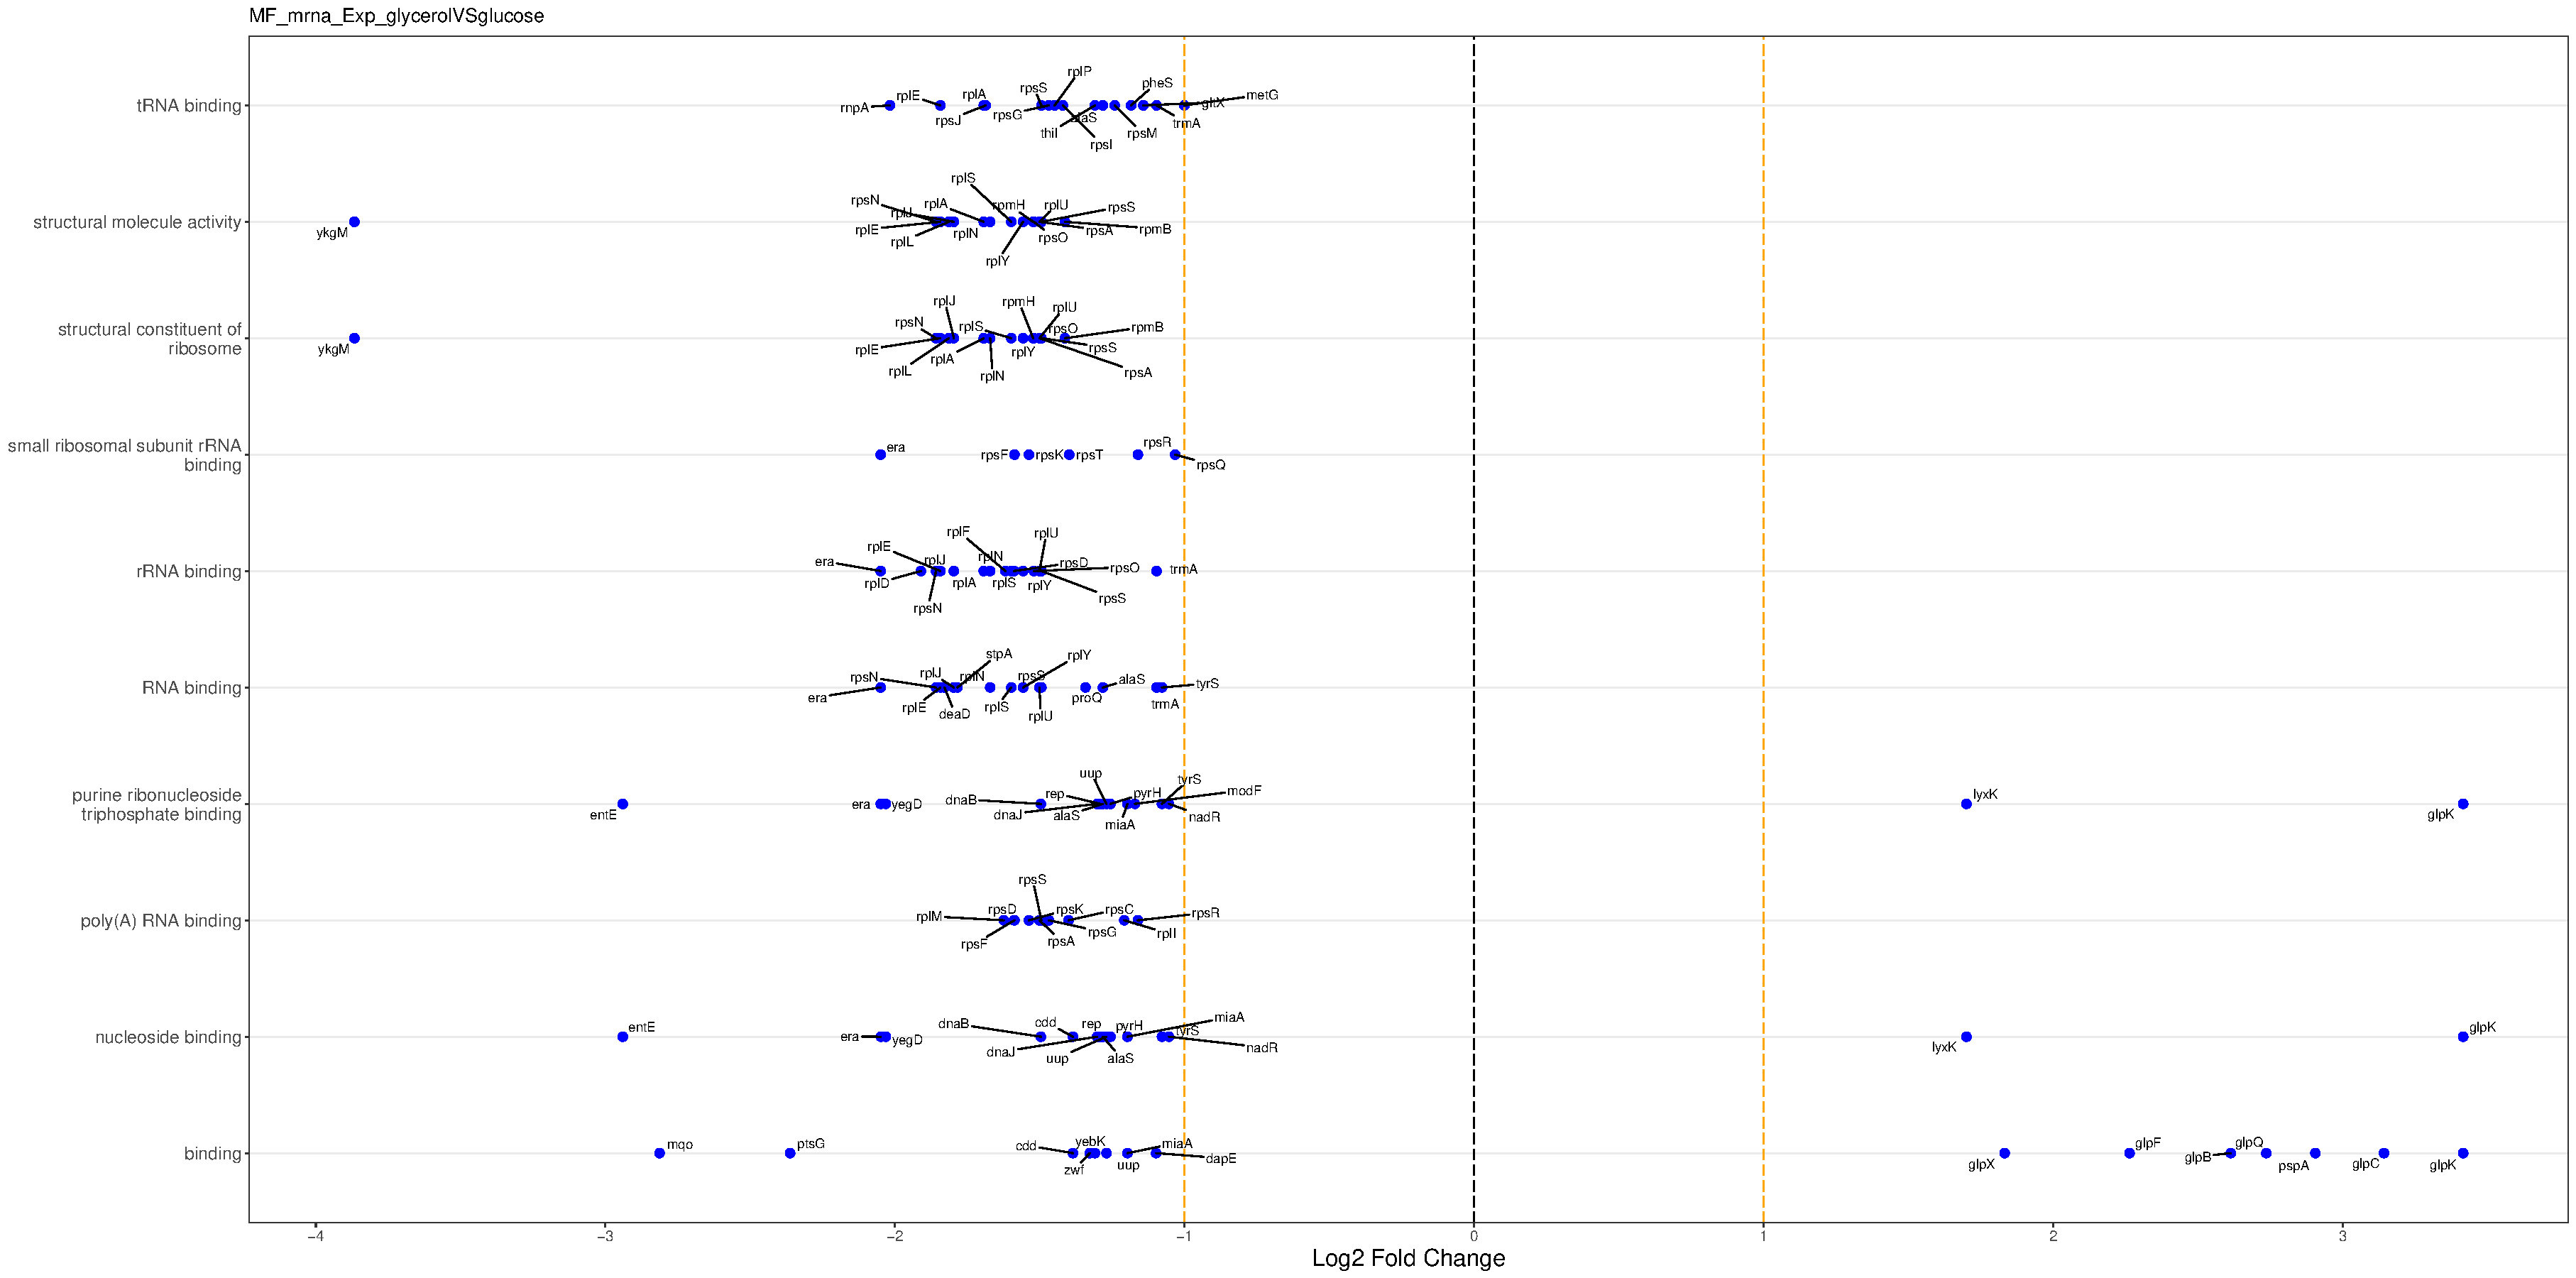
\includegraphics[width=1.0\textwidth]{../../d_figures/MF01_mrna_Exp_glycerolVSglucose_withTitle.pdf}
	\caption[Significantly differentially expressed GO annotations associated with molecular functions for mRNA samples in exponential phase tested for glycerol against glucose]
	{\textbf{Significantly differentially expressed GO annotations related with molecular functions and associated genes with glycerol as carbon source, as determined by mRNA abundances in exponential phase.} The top 10 differentially expressed molecular functions are shown along the $y$ axis, and the relative fold change of the corresponding genes is shown along the $x$ axis. We show up to 10 of the most significantly changed molecular functions and for each molecular function, we show up to 15 of the most significantly changing genes.}
\end{figure}


\begin{figure}[!htb]
	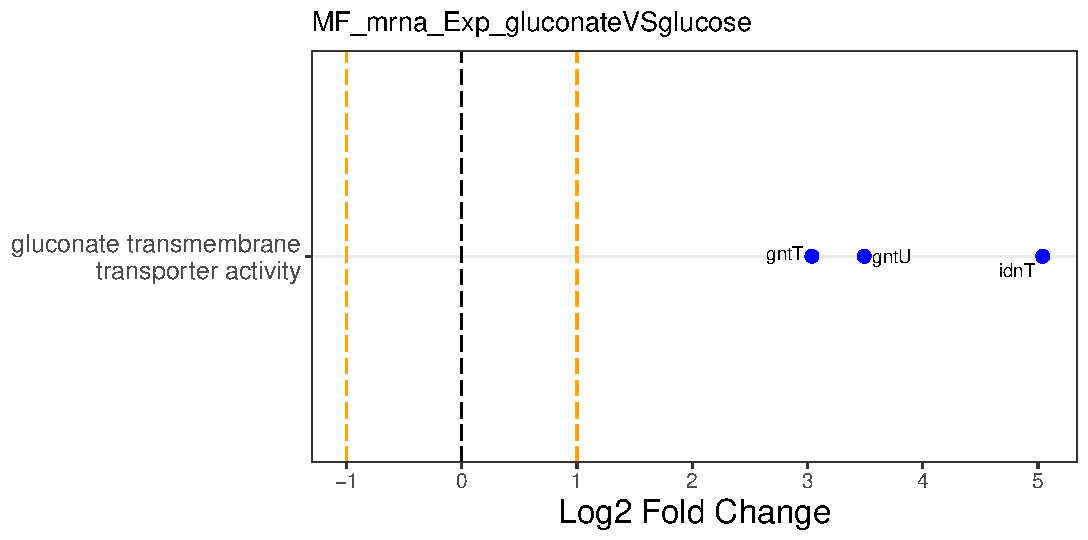
\includegraphics[width=1.0\textwidth]{../../d_figures/MF02_mrna_Exp_gluconateVSglucose_withTitle.pdf}
	\caption[Significantly differentially expressed GO annotations associated with molecular functions for mRNA samples in exponential phase tested for gluconate against glucose]
	{\textbf{Significantly differentially expressed GO annotations related with molecular functions and associated genes with gluconate as carbon source, as determined by mRNA abundances in exponential phase.} The top 2 differentially expressed molecular functions are shown along the $y$ axis, and the relative fold change of the corresponding genes is shown along the $x$ axis. We show up to 10 of the most significantly changed molecular functions and for each molecular function, we show up to 15 of the most significantly changing genes.}
\end{figure}

\begin{figure}[!htb]
	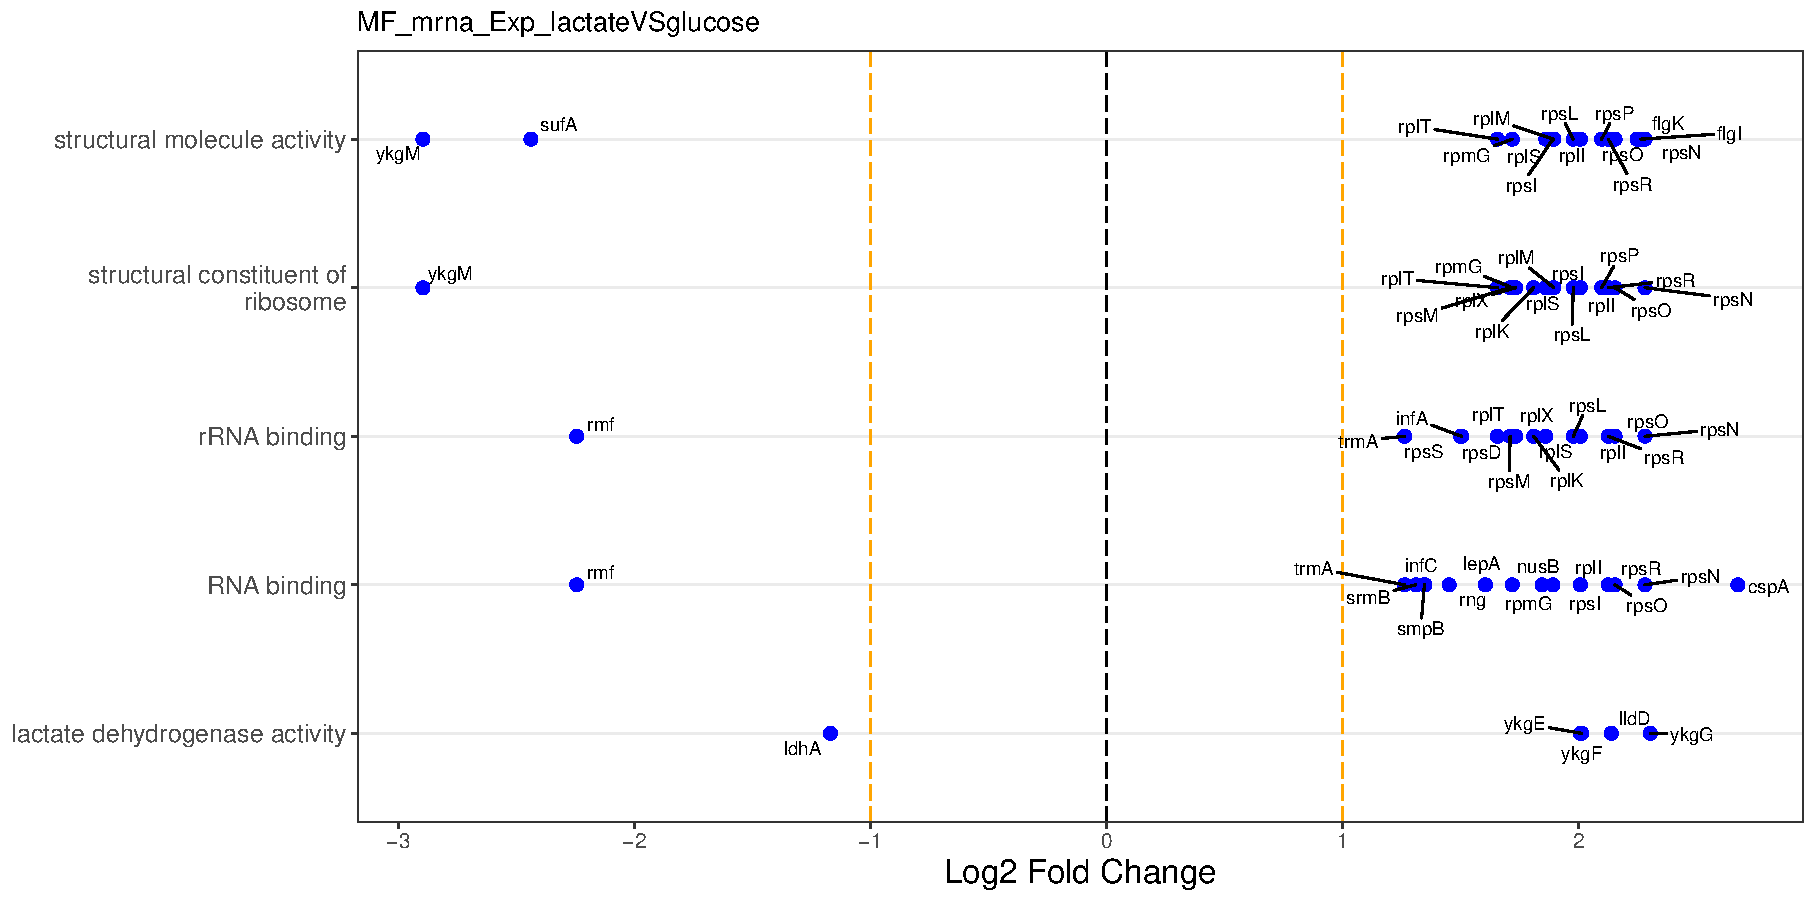
\includegraphics[width=1.0\textwidth]{../../d_figures/MF03_mrna_Exp_lactateVSglucose_withTitle.pdf}
	\caption[Significantly differentially expressed GO annotations associated with molecular functions for mRNA samples in exponential phase tested for lactate against glucose]
	{\textbf{Significantly differentially expressed GO annotations related with molecular functions and associated genes with lactate as carbon source, as determined by mRNA abundances in exponential phase.} The top 5 differentially expressed molecular functions are shown along the $y$ axis, and the relative fold change of the corresponding genes is shown along the $x$ axis. We show up to 10 of the most significantly changed molecular functions and for each molecular function, we show up to 15 of the most significantly changing genes.}
\end{figure}


\begin{figure}[!htb]
	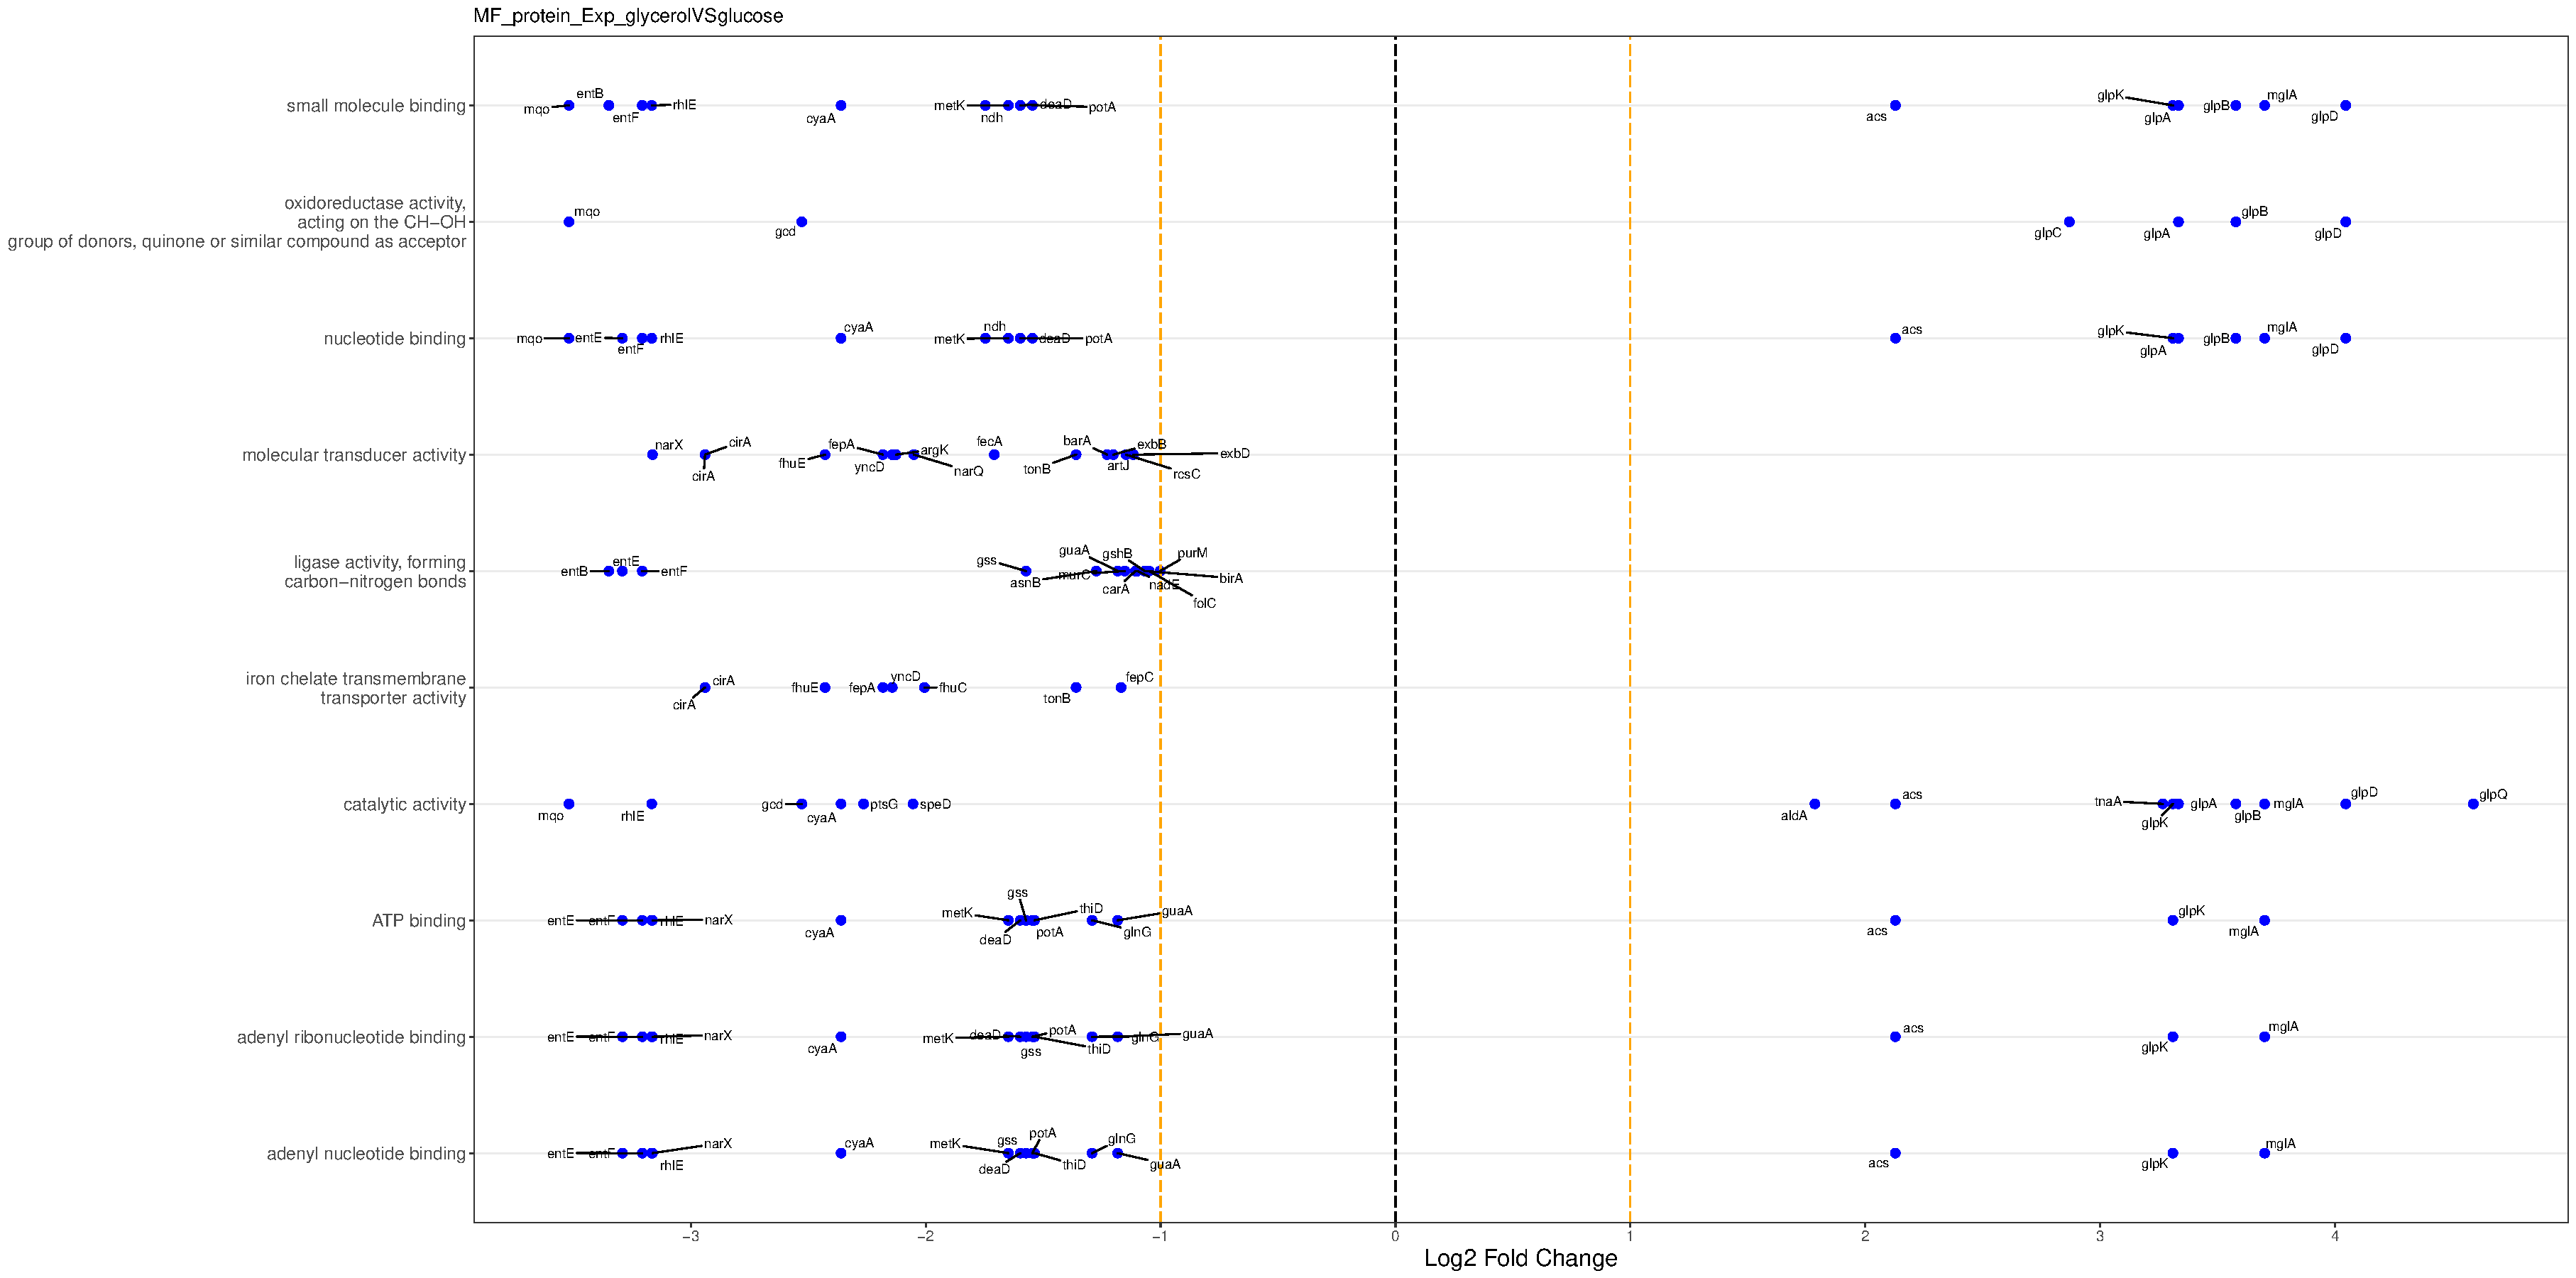
\includegraphics[width=1.0\textwidth]{../../d_figures/MF04_protein_Exp_glycerolVSglucose_withTitle.pdf}
	\caption[Significantly differentially expressed GO annotations associated with molecular functions for protein samples in exponential phase tested for glycerol against glucose]
	{\textbf{Significantly differentially expressed GO annotations related with molecular functions and associated genes with glycerol as carbon source, as determined by protein abundances in exponential phase.} The top 10 differentially expressed molecular functions are shown along the $y$ axis, and the relative fold change of the corresponding genes is shown along the $x$ axis. We show up to 10 of the most significantly changed molecular functions and for each molecular function, we show up to 15 of the most significantly changing genes.}
\end{figure}


\begin{figure}[!htb]
	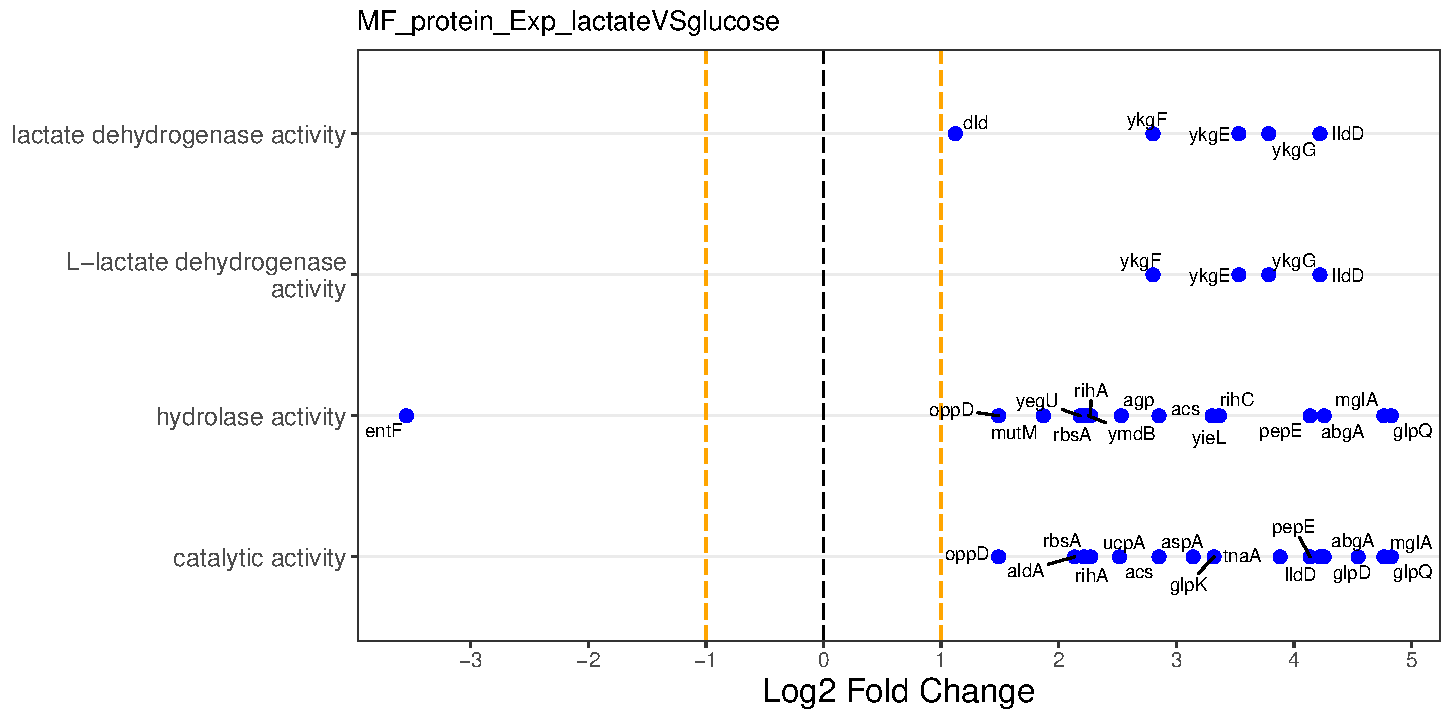
\includegraphics[width=1.0\textwidth]{../../d_figures/MF05_protein_Exp_lactateVSglucose_withTitle.pdf}
	\caption[Significantly differentially expressed GO annotations associated with molecular functions for protein samples in exponential phase tested for lactate against glucose]
	{\textbf{Significantly differentially expressed GO annotations related with molecular functions and associated genes with lactate as carbon source, as determined by protein abundances in exponential phase.} The top 4 differentially expressed molecular functions are shown along the $y$ axis, and the relative fold change of the corresponding genes is shown along the $x$ axis. We show up to 10 of the most significantly changed molecular functions and for each molecular function, we show up to 15 of the most significantly changing genes.}
\end{figure}


\begin{figure}[!htb]
	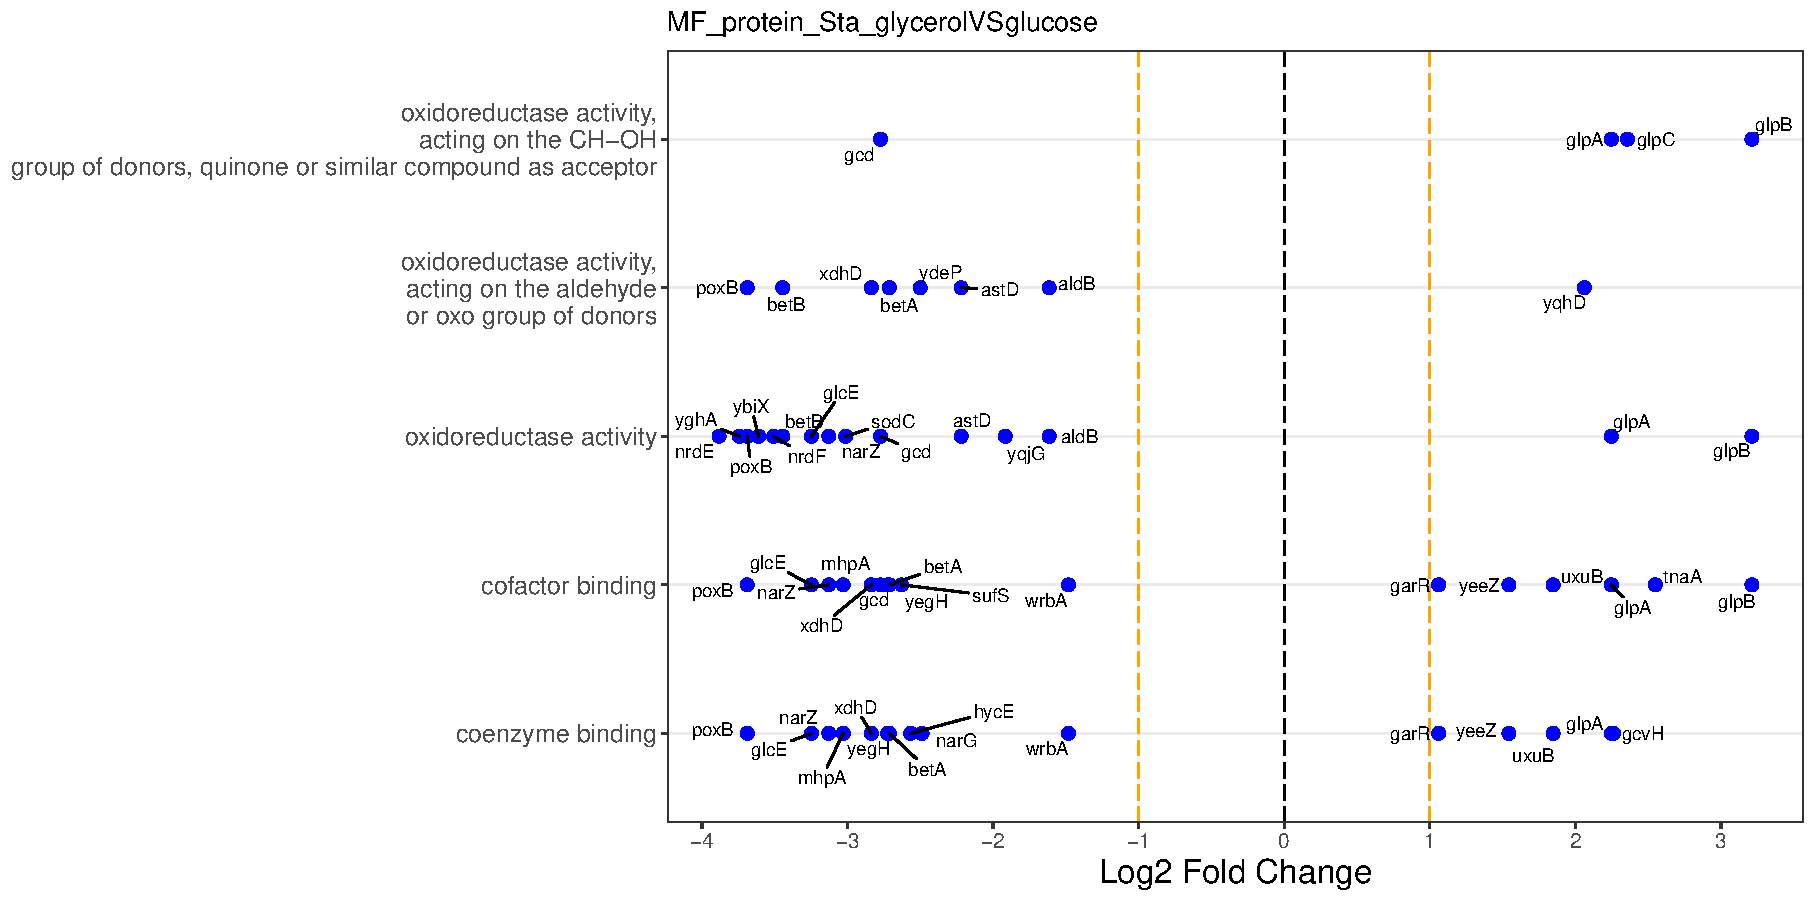
\includegraphics[width=1.0\textwidth]{../../d_figures/MF06_protein_Sta_glycerolVSglucose_withTitle.pdf}
	\caption[Significantly differentially expressed GO annotations associated with molecular functions for protein samples in stationary phase tested for glycerol against glucose]
	{\textbf{Significantly differentially expressed GO annotations related with molecular functions and associated genes with glycerol as carbon source, as determined by protein abundances in stationary phase.} The top 5 differentially expressed molecular functions are shown along the $y$ axis, and the relative fold change of the corresponding genes is shown along the $x$ axis. We show up to 10 of the most significantly changed molecular functions and for each molecular function, we show up to 15 of the most significantly changing genes.}
\end{figure}

\begin{figure}[!htb]
	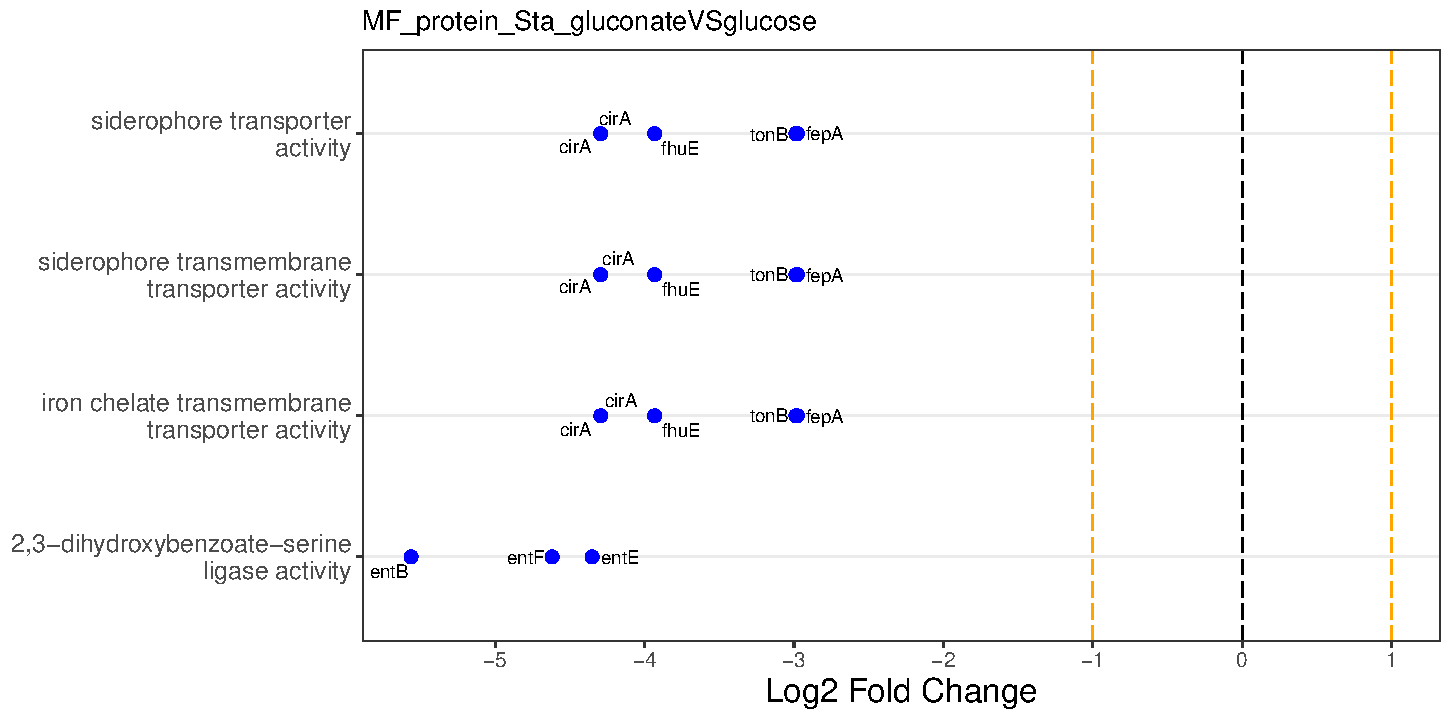
\includegraphics[width=1.0\textwidth]{../../d_figures/MF07_protein_Sta_gluconateVSglucose_withTitle.pdf}
	\caption[Significantly differentially expressed GO annotations associated with molecular functions for protein samples in stationary phase tested for gluconate against glucose]
	{\textbf{Significantly differentially expressed GO annotations related with molecular functions and associated genes with gluconate as carbon source, as determined by protein abundances in stationary phase.} The top 4 differentially expressed molecular functions are shown along the $y$ axis, and the relative fold change of the corresponding genes is shown along the $x$ axis. We show up to 10 of the most significantly changed molecular functions and for each molecular function, we show up to 15 of the most significantly changing genes.}
\end{figure}

\begin{figure}[!htb]
	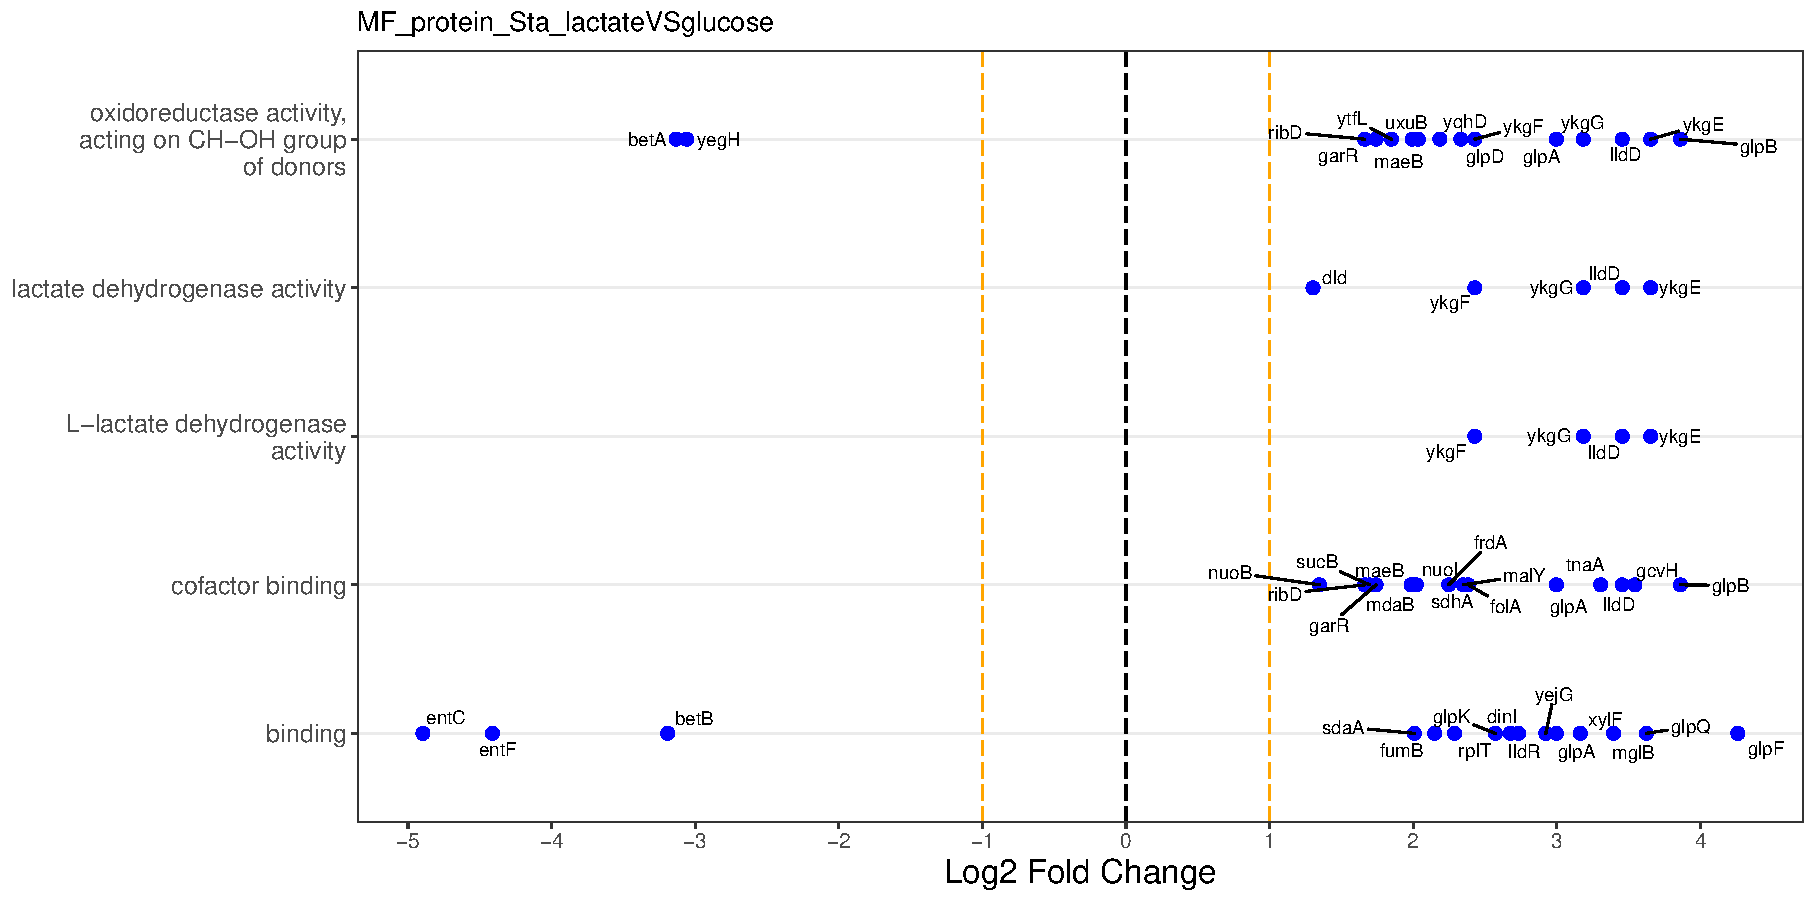
\includegraphics[width=1.0\textwidth]{../../d_figures/MF08_protein_Sta_lactateVSglucose_withTitle.pdf}
	\caption[Significantly differentially expressed GO annotations associated with molecular functions for protein samples in stationary phase tested for lactate against glucose]
	{\textbf{Significantly differentially expressed GO annotations related with molecular functions and associated genes with lactate as carbon source, as determined by protein abundances in stationary phase.} The top 5 differentially expressed molecular functions are shown along the $y$ axis, and the relative fold change of the corresponding genes is shown along the $x$ axis. We show up to 10 of the most significantly changed molecular functions and for each molecular function, we show up to 15 of the most significantly changing genes.}
\end{figure}

\begin{figure}[!htb]
	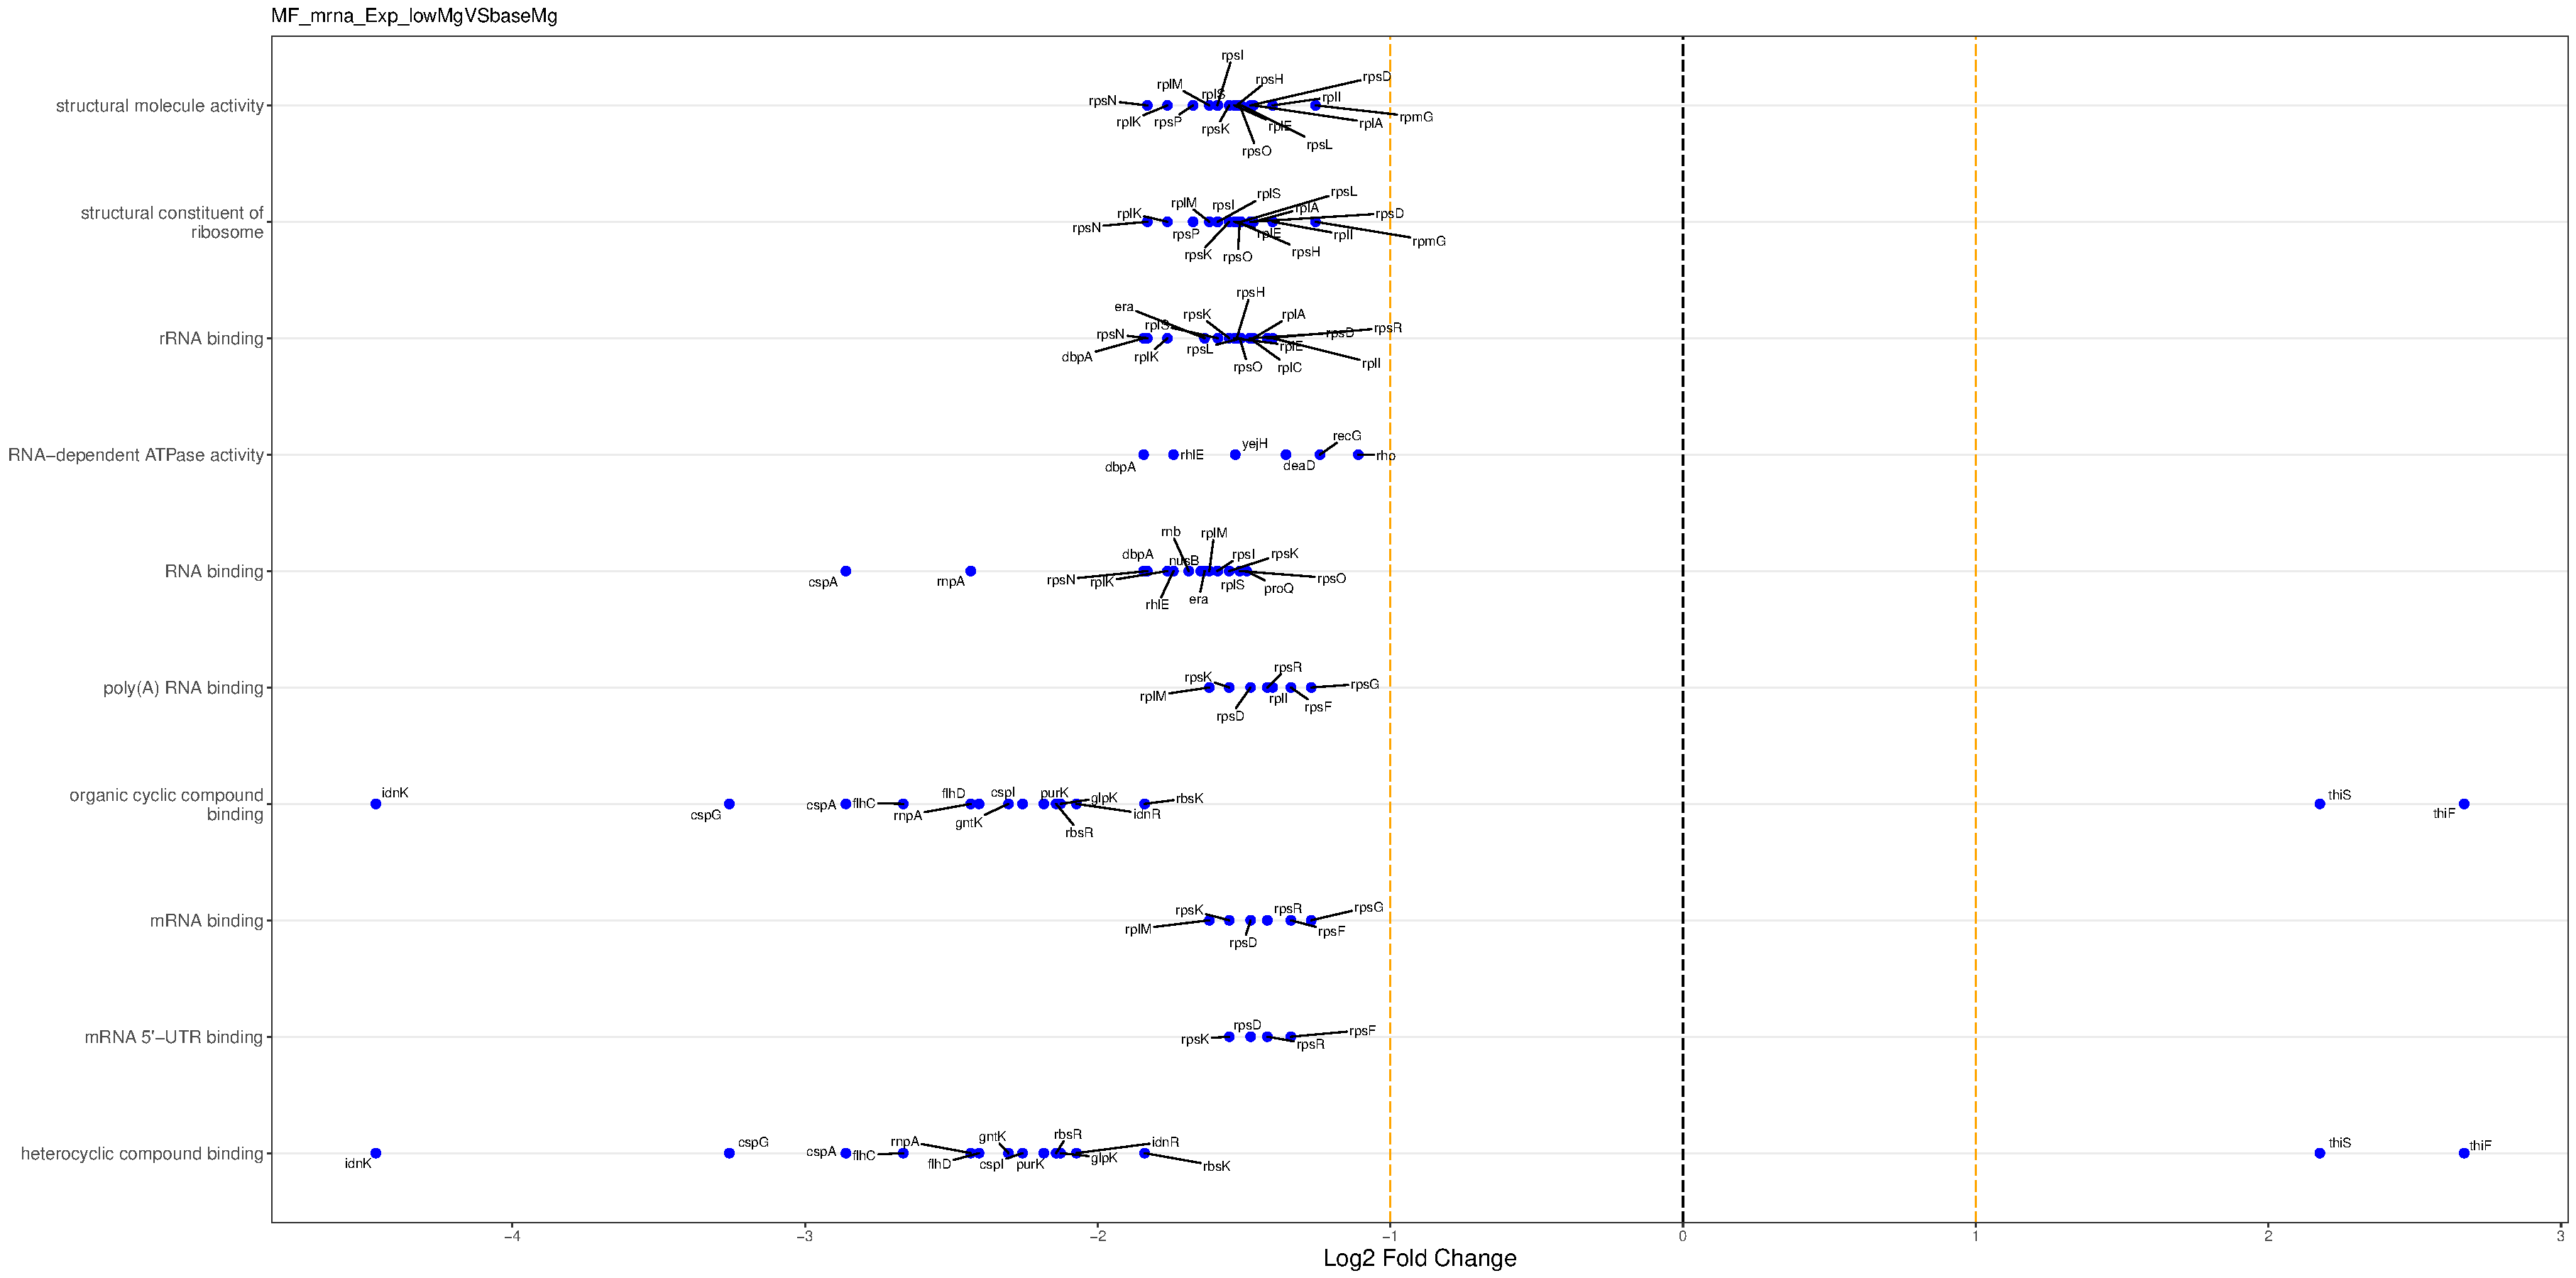
\includegraphics[width=1.0\textwidth]{../../d_figures/MF09_mrna_Exp_lowMgVSbaseMg_withTitle.pdf}
	\caption[Significantly differentially expressed GO annotations associated with molecular functions for mRNA samples in exponential phase tested for low Mg\textsuperscript{2+} levels against base Mg\textsuperscript{2+} levels]
	{\textbf{Significantly differentially expressed GO annotations related with molecular functions and associated genes with low Mg\textsuperscript{2+} levels, as determined by mRNA abundances in exponential phase.} The top 10 differentially expressed molecular functions are shown along the $y$ axis, and the relative fold change of the corresponding genes is shown along the $x$ axis. We show up to 10 of the most significantly changed molecular functions and for each molecular function, we show up to 15 of the most significantly changing genes.}
\end{figure}

\begin{figure}[!htb]
	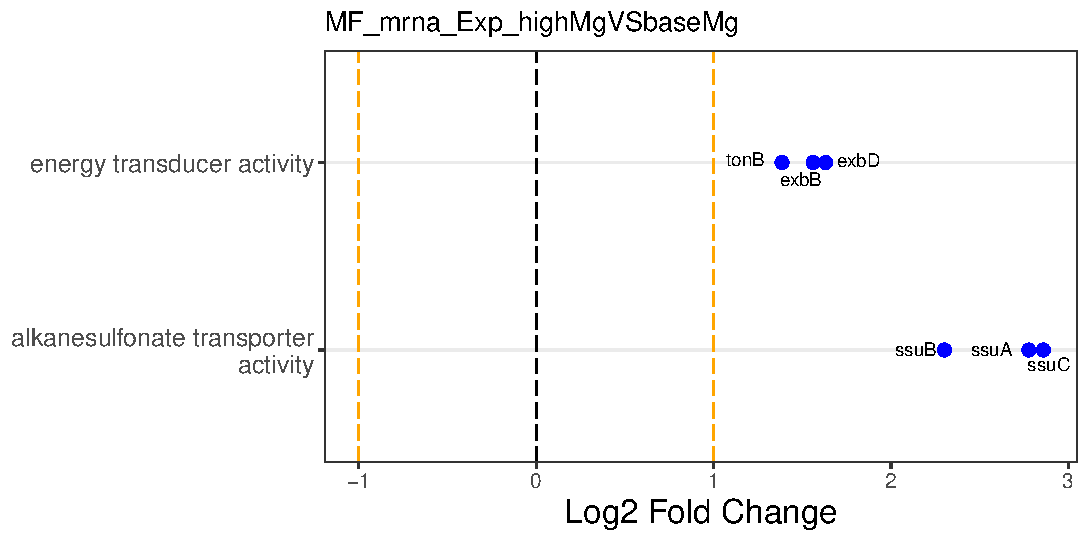
\includegraphics[width=1.0\textwidth]{../../d_figures/MF10_mrna_Exp_highMgVSbaseMg_withTitle.pdf}
	\caption[Significantly differentially expressed GO annotations associated with molecular functions for mRNA samples in exponential phase tested for high Mg\textsuperscript{2+} levels against base Mg\textsuperscript{2+} levels]
	{\textbf{Significantly differentially expressed GO annotations related with molecular functions and associated genes with high Mg\textsuperscript{2+} levels, as determined by mRNA abundances in exponential phase.} The top 3 differentially expressed molecular functions are shown along the $y$ axis, and the relative fold change of the corresponding genes is shown along the $x$ axis. We show up to 10 of the most significantly changed molecular functions and for each molecular function, we show up to 15 of the most significantly changing genes.}
\end{figure}

\begin{figure}[!htb]
	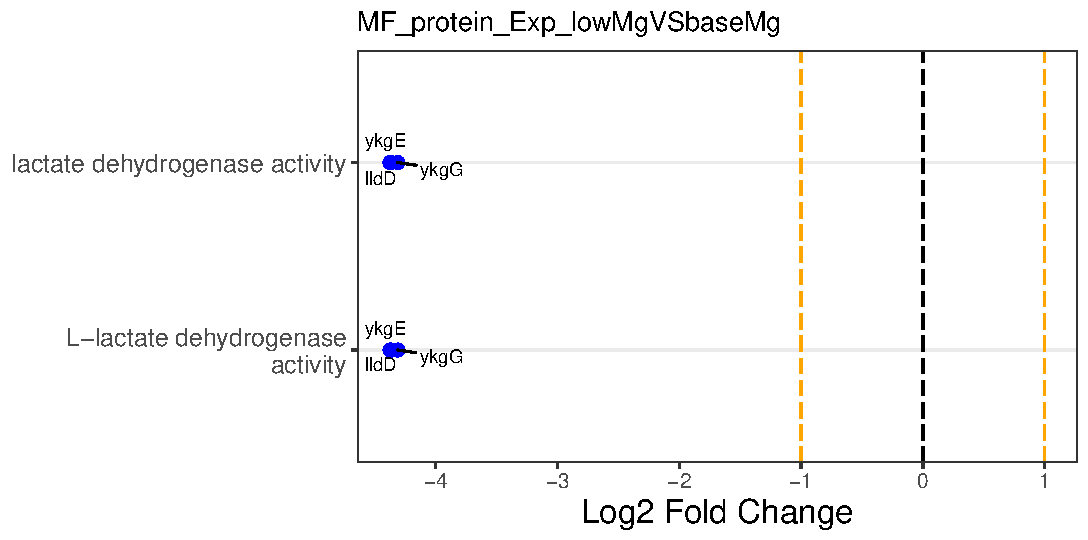
\includegraphics[width=1.0\textwidth]{../../d_figures/MF11_protein_Exp_lowMgVSbaseMg_withTitle.pdf}
	\caption[Significantly differentially expressed GO annotations associated with molecular functions for protein samples in exponential phase tested for low Mg\textsuperscript{2+} levels against base Mg\textsuperscript{2+} levels]
	{\textbf{Significantly differentially expressed GO annotations related with molecular functions and associated genes with low Mg\textsuperscript{2+} levels, as determined by protein abundances in exponential phase.} The top 2 differentially expressed molecular functions are shown along the $y$ axis, and the relative fold change of the corresponding genes is shown along the $x$ axis. We show up to 10 of the most significantly changed molecular functions and for each molecular function, we show up to 15 of the most significantly changing genes.}
\end{figure}

\begin{figure}[!htb]
	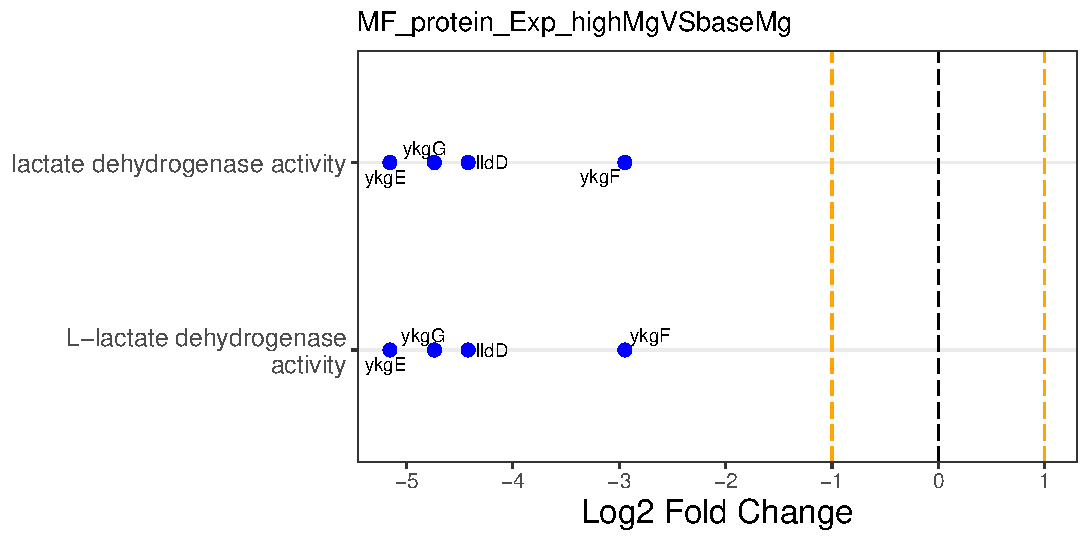
\includegraphics[width=1.0\textwidth]{../../d_figures/MF12_protein_Exp_highMgVSbaseMg_withTitle.pdf}
	\caption[Significantly differentially expressed GO annotations associated with molecular functions for protein samples in exponential phase tested for high Mg\textsuperscript{2+} levels against base Mg\textsuperscript{2+} levels]
	{\textbf{Significantly differentially expressed GO annotations related with molecular functions and associated genes with high Mg\textsuperscript{2+} levels, as determined by protein abundances in exponential phase.} The top 2 differentially expressed molecular functions are shown along the $y$ axis, and the relative fold change of the corresponding genes is shown along the $x$ axis. We show up to 10 of the most significantly changed molecular functions and for each molecular function, we show up to 15 of the most significantly changing genes.}
\end{figure}

\begin{figure}[!htb]
	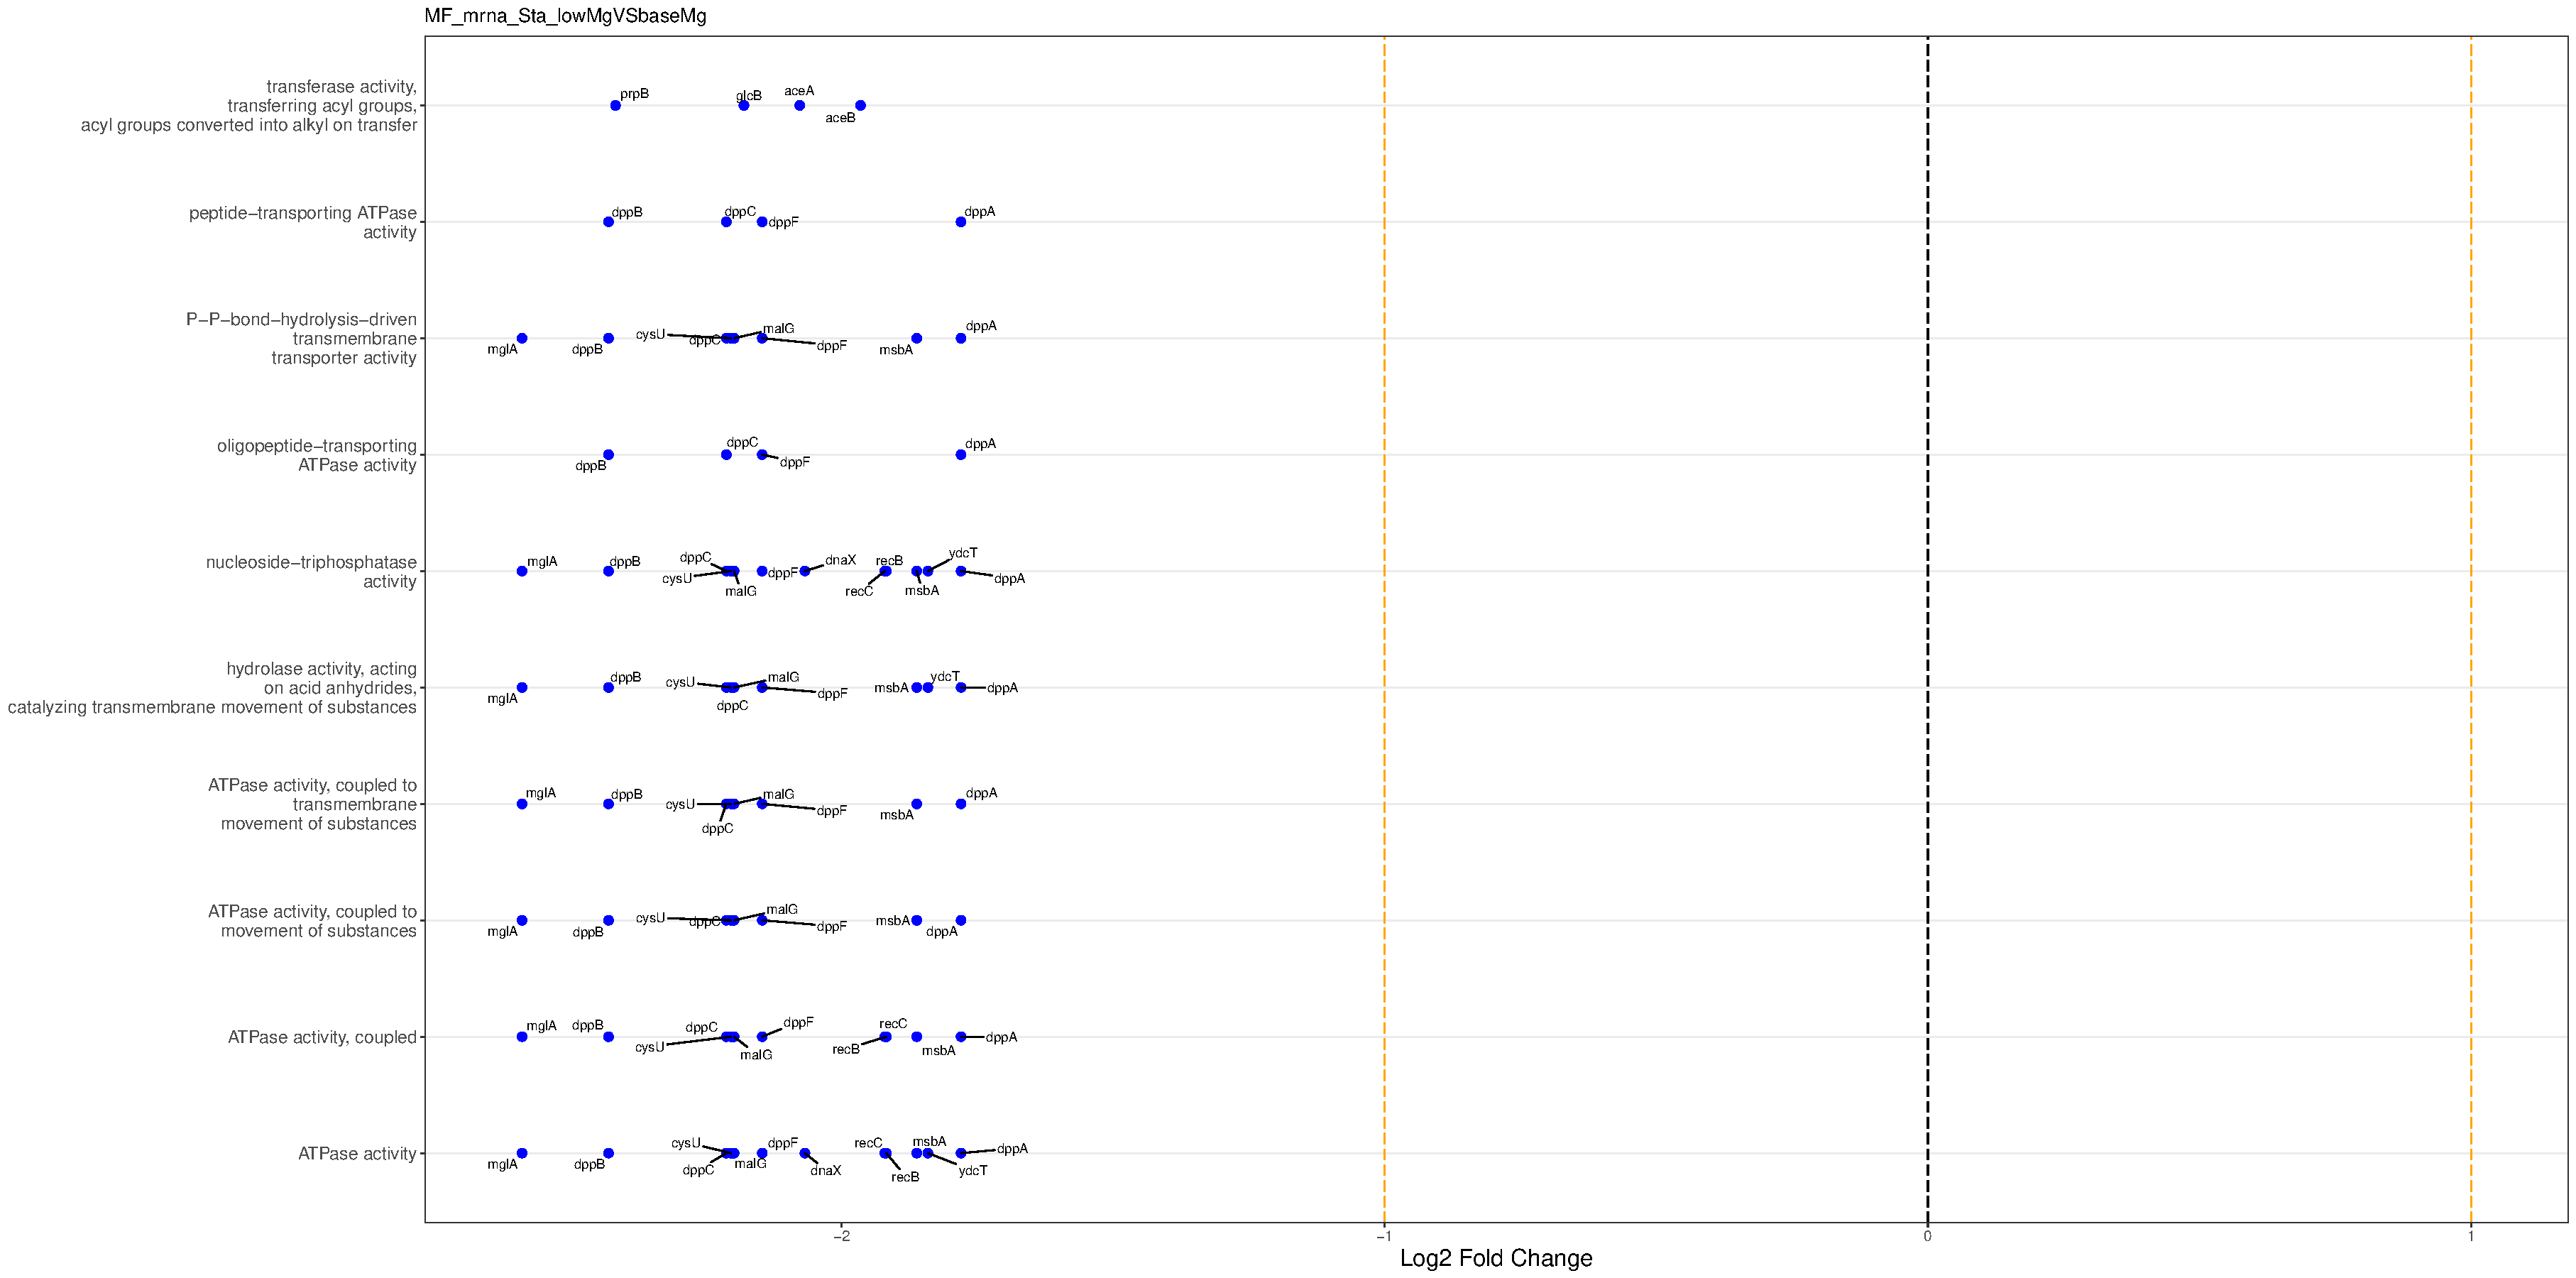
\includegraphics[width=1.0\textwidth]{../../d_figures/MF13_mrna_Sta_lowMgVSbaseMg_withTitle.pdf}
	\caption[Significantly differentially expressed GO annotations associated with molecular functions for mRNA samples in stationary phase tested for low Mg\textsuperscript{2+} levels against base Mg\textsuperscript{2+} levels]
	{\textbf{Significantly differentially expressed GO annotations related with molecular functions and associated genes with low Mg\textsuperscript{2+} levels, as determined by mRNA abundances in stationary phase.} The top 10 differentially expressed molecular functions are shown along the $y$ axis, and the relative fold change of the corresponding genes is shown along the $x$ axis. We show up to 10 of the most significantly changed molecular functions and for each molecular function, we show up to 15 of the most significantly changing genes.}
\end{figure}

\begin{figure}[!htb]
	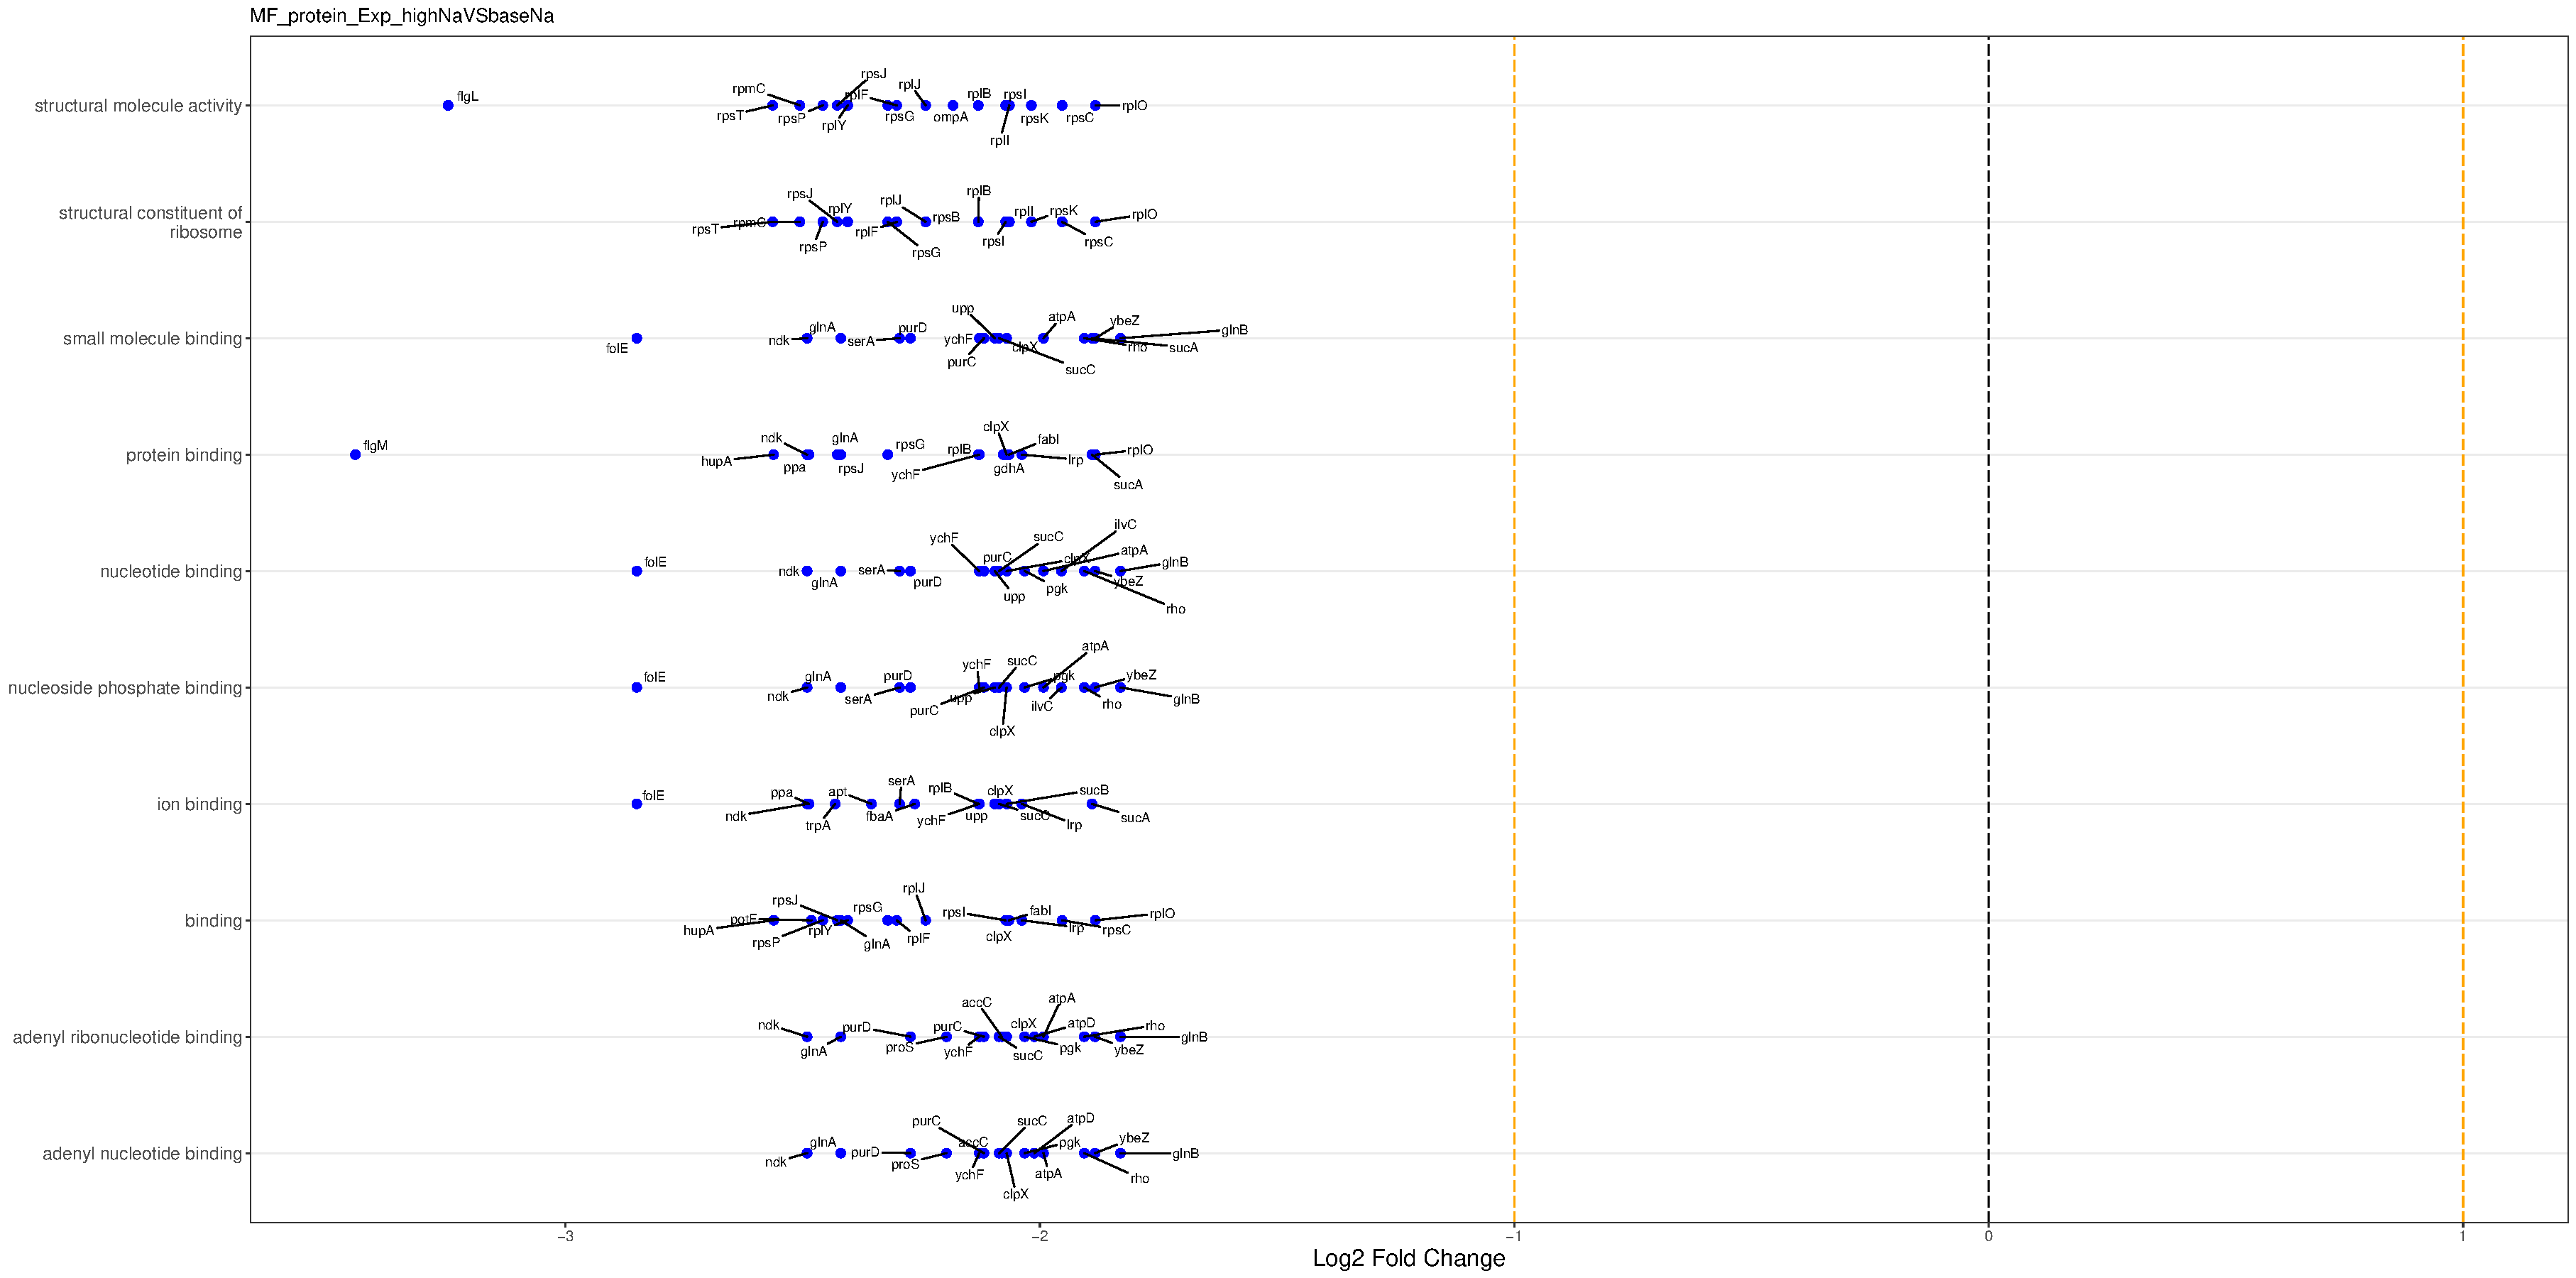
\includegraphics[width=1.0\textwidth]{../../d_figures/MF14_protein_Exp_highNaVSbaseNa_withTitle.pdf}
	\caption[Significantly differentially expressed GO annotations associated with molecular functions for protein samples in exponential phase tested for high Na\textsuperscript{+} levels against base Na\textsuperscript{+} levels]
	{\textbf{Significantly differentially expressed GO annotations related with molecular functions and associated genes with high Na\textsuperscript{+} levels, as determined by protein abundances in exponential phase.} The top differentially expressed molecular functions are shown along the $y$ axis, and the relative fold change of the corresponding genes is shown along the $x$ axis. We show up to 10 of the most significantly changed molecular functions and for each molecular function, we show up to 15 of the most significantly changing genes.}
\end{figure}

\begin{figure}[!htb]
	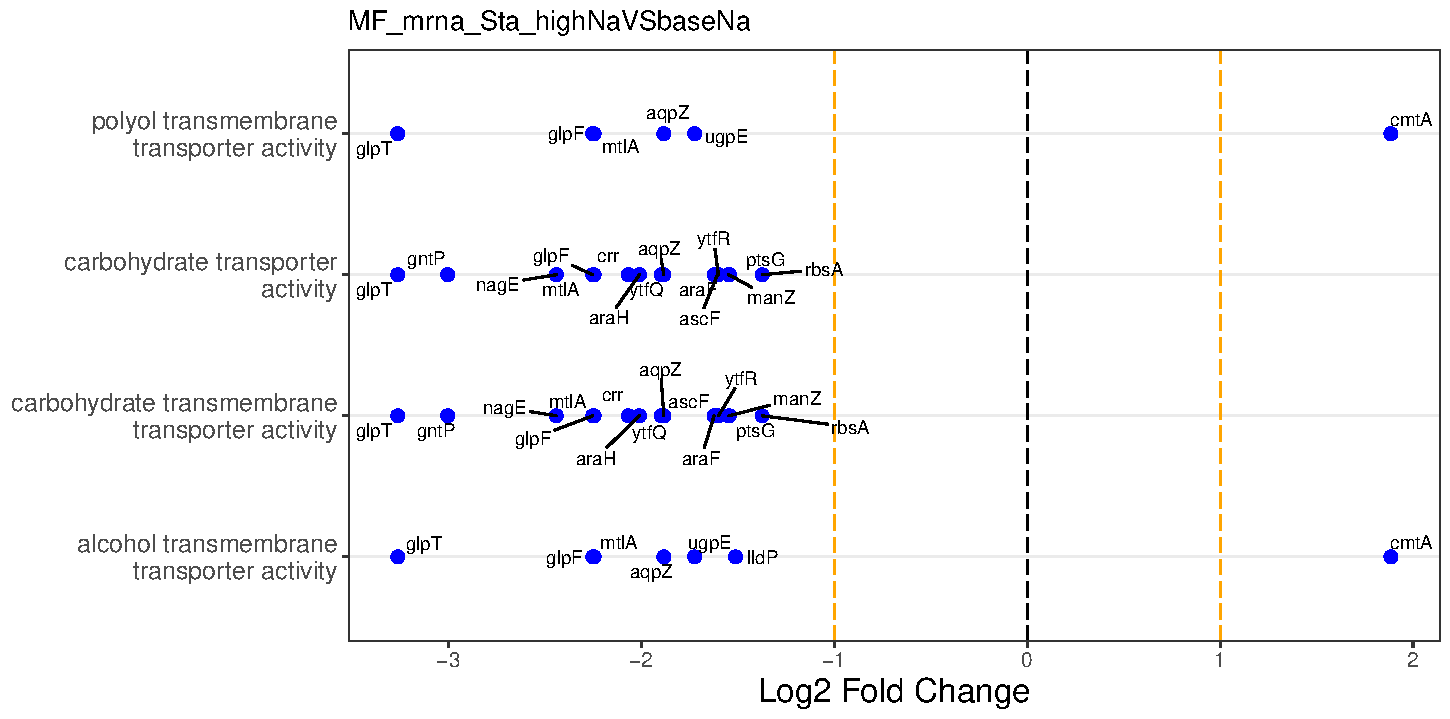
\includegraphics[width=1.0\textwidth]{../../d_figures/MF15_mrna_Sta_highNaVSbaseNa_withTitle.pdf}
	\caption[Significantly differentially expressed GO annotations associated with molecular functions for mRNA samples in stationary phase tested for high Na\textsuperscript{+} levels against base Na\textsuperscript{+} levels]
	{\textbf{Significantly differentially expressed GO annotations related with molecular functions and associated genes with high Na\textsuperscript{+} levels, as determined by mRNA abundances in stationary phase.} The top 5 differentially expressed molecular functions are shown along the $y$ axis, and the relative fold change of the corresponding genes is shown along the $x$ axis. We show up to 10 of the most significantly changed molecular functions and for each molecular function, we show up to 15 of the most significantly changing genes.}
\end{figure}

\begin{figure}[!htb]
	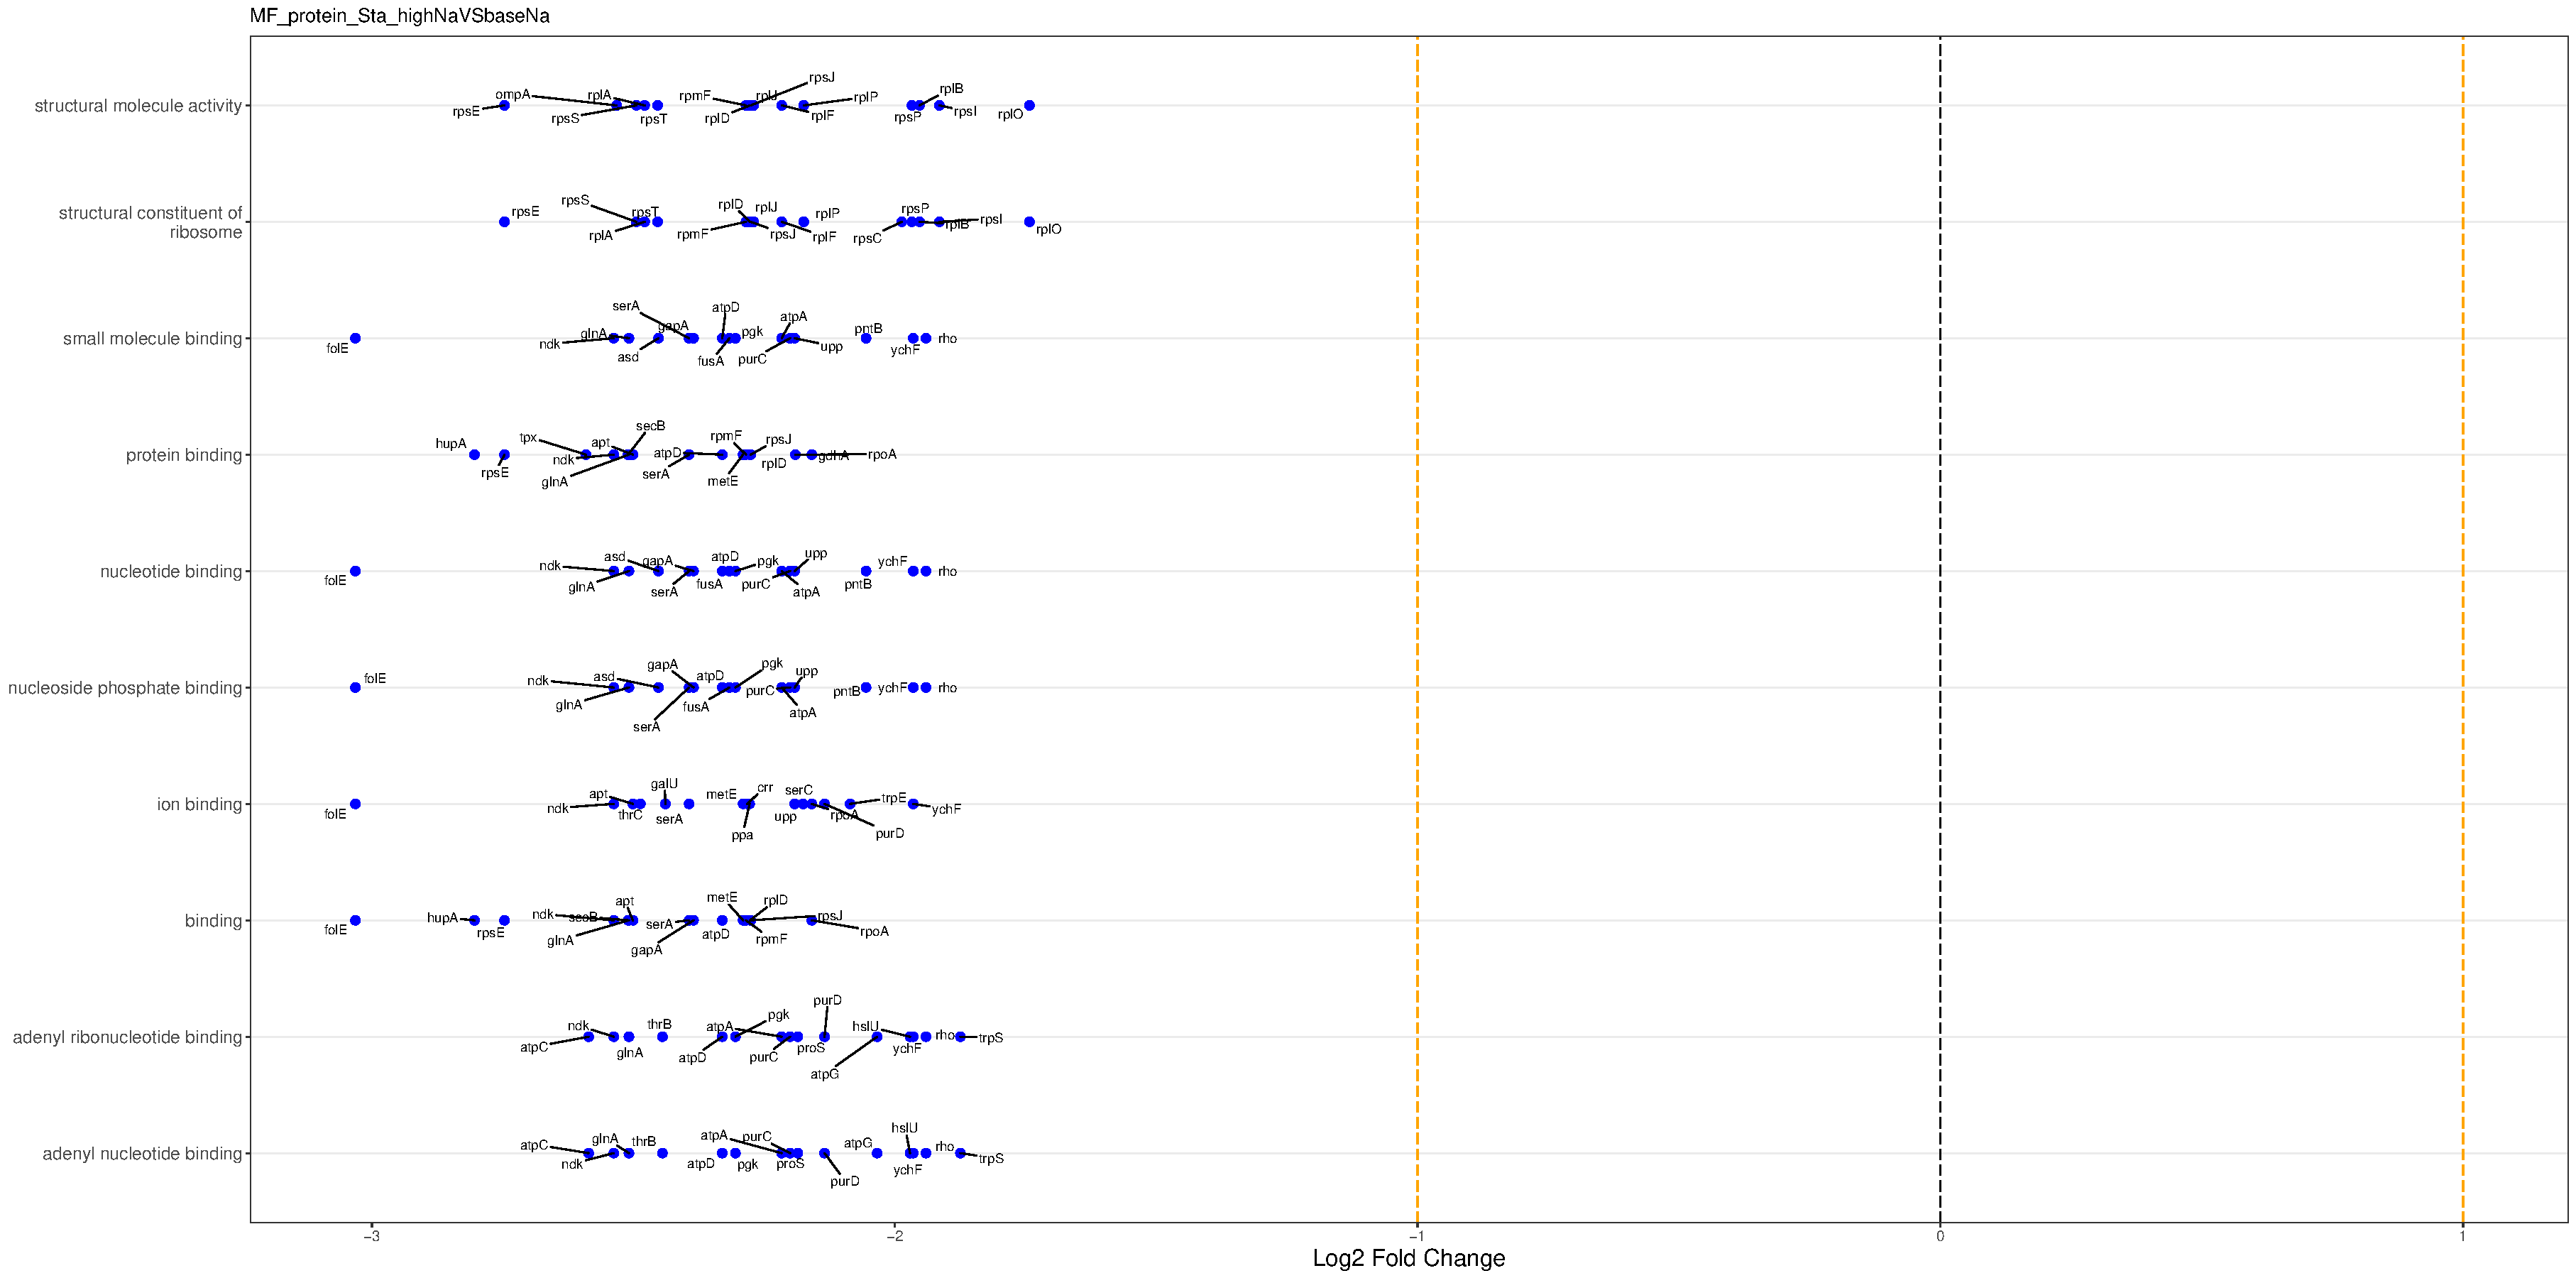
\includegraphics[width=1.0\textwidth]{../../d_figures/MF16_protein_Sta_highNaVSbaseNa_withTitle.pdf}
	\caption[Significantly differentially expressed GO annotations associated with molecular functions for protein samples in stationary phase tested for high Na\textsuperscript{+} levels against base Na\textsuperscript{+} levels]
	{\textbf{Significantly differentially expressed GO annotations related with molecular functions and associated genes with high Na\textsuperscript{+} levels, as determined by protein abundances in stationary phase.} The top 10 differentially expressed molecular functions are shown along the $y$ axis, and the relative fold change of the corresponding genes is shown along the $x$ axis. We show up to 10 of the most significantly changed molecular functions and for each molecular function, we show up to 15 of the most significantly changing genes.}
\end{figure}





\clearpage
\begin{figure}[!htb]
	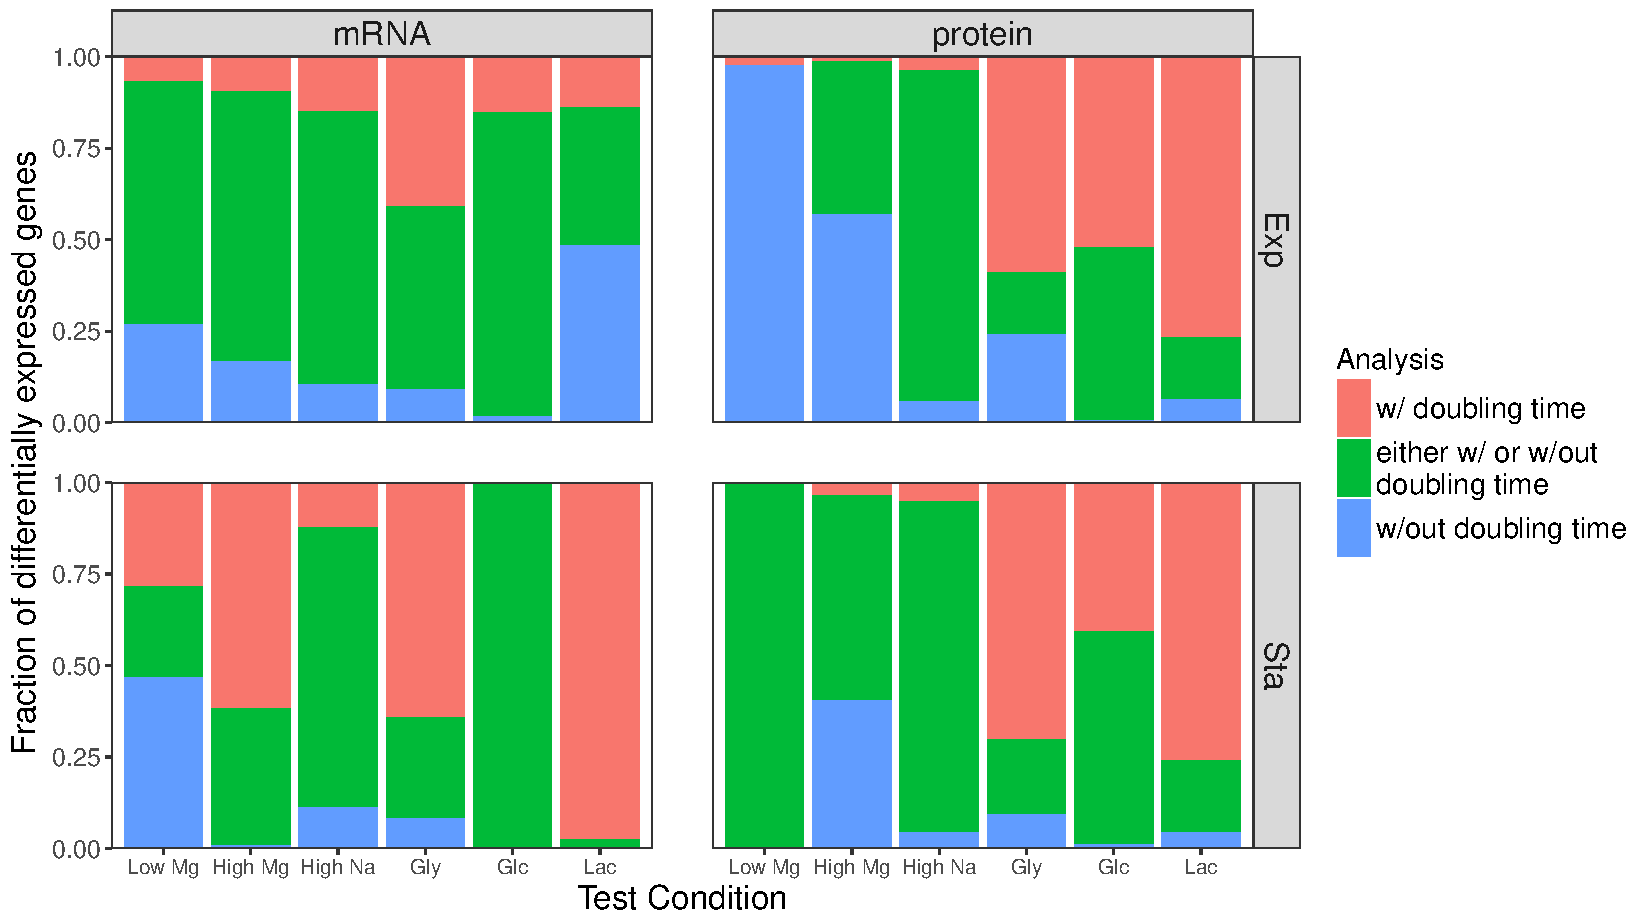
\includegraphics[width=1\textwidth]{../../c_figures/difference_rtw_GrowthControl.pdf}
	\caption[Fraction of differentially expressed genes that are found in analyses with or without controlling for doubling time]
	{\textbf{Fraction of differentially expressed genes that are found in analyses with or without controlling for doubling time.} Shown are the fractions of genes identified as differentially expressed only when controlling for doubling time (red), only when not controlling for doubling time (blue), or in both cases (green). Combined with the absolute numbers of differentially expressed genes in the various conditions (Figure 5), we can see that the main differences in analyses with or without doubling time arise for protein abundances analyzed with respect to different carbon sources.}
\end{figure}




\clearpage
\begin{figure}[!htb]
	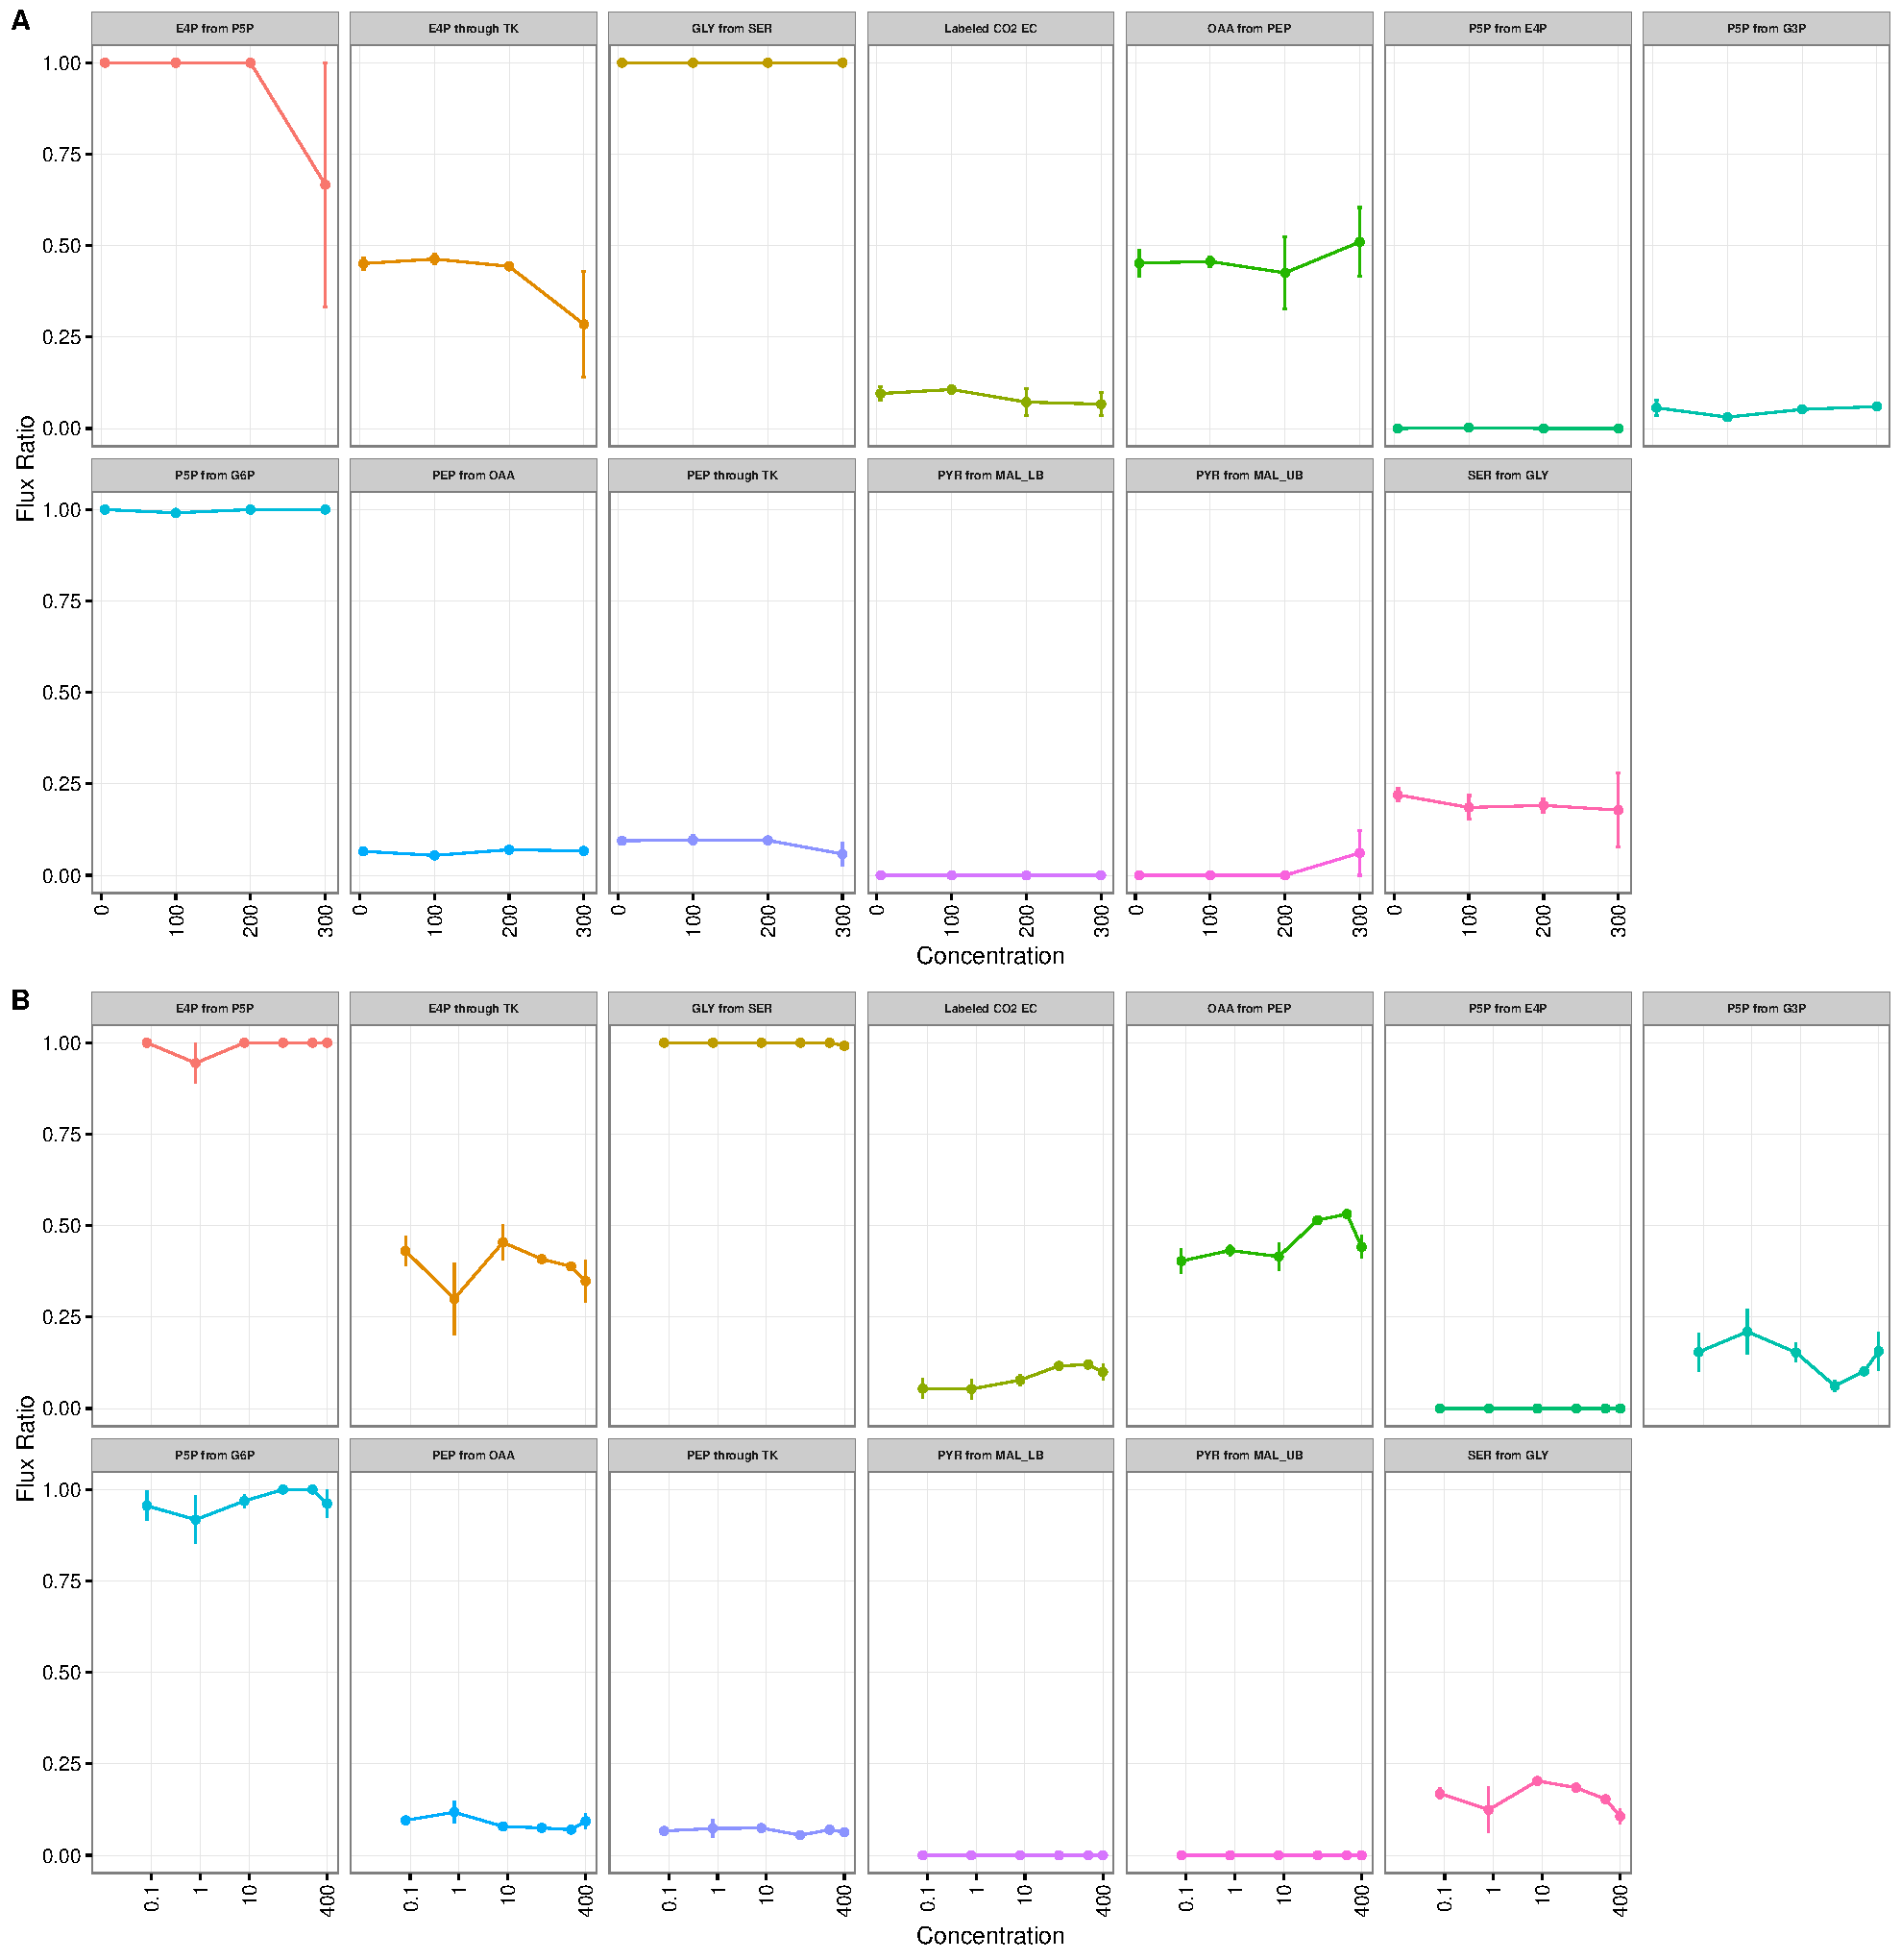
\includegraphics[width=1\textwidth]{../../e_figures/Exp.pdf}
	\caption[Flux ratios versus ion concentrations]
	{\textbf{Flux ratios versus ion concentrations.} 13 different flux ratios were measured with respect to four different Na\textsuperscript{+} and five different Mg\textsuperscript{2+} concentrations. (A) Concentrations with respect to changing Na+ concentrations. (B) Concentrations with respect to changing Mg\textsuperscript{2+} concentrations. There was no significant trend of increase or decrease in flux ratios with respect to either Na\textsuperscript{+} or Mg\textsuperscript{2+} concentrations (Supplementary Table 13).}
\end{figure}




\clearpage

\section*{List of Supplementary Tables}

\paragraph*{Supplementary Table S1:} 
Meta information for each sample. Includes information about sample numbers, experiment, the growth time at which the sample was collected, harvest date, number of RNA samples (technical replicates), number of protein samples (technical replicates), batch number, Mg\textsuperscript{2+} and Na\textsuperscript{+} concentrations, growth phase, doubling time (mean, $\pm95\%$ confidence interval, $r^2$ from the linear fit to OD600 values).\\

\noindent File name: tableS1\_meta\_data.csv

\paragraph*{Supplementary Table S2:} Normalized mRNA counts. Includes data for 4196 distinct proteins each for 152 samples.\\

\noindent File name: tableS2\_mRNA\_normalized\_raw\_data.csv

\paragraph*{Supplementary Table S3:} Normalized protein counts. Includes data for 4196 distinct proteins each for 105 samples.\\

\noindent File name: tableS3\_protein\_normalized\_raw\_data.csv


\paragraph*{Supplementary Table S4:} Mean flux ratios for 13 branches each, measured for varying Mg\textsuperscript{2+} and Na\textsuperscript{+} concentrations in exponential and stationary phase.\\

\noindent File name: tableS4\_fluxData.csv


\paragraph*{Supplementary Table S5:} Doubling time measurements in exponential phase. Includes the mean, $\pm95\%$ confidence interval, and $r^2$ from the linear fit to OD600 values.\\

\noindent File name: tableS5\_doubling\_times.csv


\paragraph*{Supplementary Table S6:} $z$-scores obtained from tests for significant clustering of mRNA counts.\\

\noindent File name: tableS6\_clustering\_mrna\_cophenetic.csv

\paragraph*{Supplementary Table S7:} $z$-scores obtained from tests for significant clustering of protein counts.\\


\noindent File name: tableS7\_clustering\_protein\_cophenetic.csv

\paragraph*{Supplementary Table S8:} Combined results from tests for differential expression for all genes and all distinct tests considered.\\
 
\noindent The table contains the following information:
\begin{itemize}
\item Gene id (ECB number for mRNA and YP number for proteins), and corresponding gene name
\item Results from DeSeq2 calculation, including base mean value, log2FoldChange, ifcSE, stat, pvalue, padj.
\item Direction of change relative to base level ("+1" for increase, "-1" for decrease)
\item Data type (mRNA or protein)
\item Growth phase
\item What is tested; base value and contrast.
\item Individual output file name 
\item Carbon Source, Mg\textsuperscript{2+} and Na\textsuperscript{+} levels and growth phase of test data 
\item Control parameters of the test (batch only or batch plus doubling time)
\end{itemize}

\noindent File name: tableS8\_combinedOutputDF\_DeSeq.csv


\paragraph*{Supplementary Table S9:} Filtered version of Supplementary Table S8, retaining only genes  with $P<0.05$ and $\text{log2FoldChange}>2$.\\

\noindent File name: tableS9\_combinedDifferentiallyExpressedGenes\_DeSeq.csv

\paragraph*{Supplementary Table S10:} Complete results from DAVID enrichment analysis for KEGG pathways and molecular functions.\\

\noindent File name: tableS10\_combinedResultList\_DAVID.csv

\paragraph*{Supplementary Table S11:} List of the additional proteins identified as differentially expressed when controlling for doubling time, tested for different carbons sources. Results are provided for both exponential and stationary phases.\\

\noindent File name: tableS11\_changed\_protein\_carbonSource\_ExpSta.csv


\paragraph*{Supplementary Table S12:} Enriched KEGG pathways and molecular functions based on the genes listed in Supplementary Table S11.\\

\noindent File name: tableS12\_changed\_DAVID\_P05.csv

\paragraph*{Supplementary Table S13:} Results from linear regressions of flux ratios against ion concentrations (Mg\textsuperscript{2+} and Na\textsuperscript{+}).\\

\noindent File name: tableS13\_flux\_vs\_conc\_Pvalues.csv


\paragraph*{Supplementary Table S14:} Results from linear regressions of flux ratios against doubling times (Mg\textsuperscript{2+} and Na\textsuperscript{+}).\\

\noindent File name: tableS14\_flux\_vs\_doublingTime\_Pvalues\_tog.csv



\end{document}
